\documentclass[12pt,a4paper]{article}
% ---------- Encodage / langue ----------
\usepackage[french]{babel}
\usepackage[utf8]{inputenc}
\usepackage[T1]{fontenc}
% ---------- Mise en page ----------
\usepackage{geometry}
\geometry{margin=2.5cm}
\setlength{\emergencystretch}{3em}
% ---------- Graphiques ----------
\usepackage{graphicx}
% Images du projet : dossier figures à la racine du dépôt et logo dans rapport/images
\graphicspath{{../figures/}{images/}}
\usepackage{xcolor}
\usepackage{tikz}
\usetikzlibrary{arrows.meta,patterns,positioning,calc,babel}
\usepackage[most]{tcolorbox}
\usepackage{float}
\usepackage{caption}
% ---------- Maths ----------
\usepackage{amsmath}
\usepackage{amssymb}
\usepackage{amsfonts}
\usepackage{algorithm}
\usepackage{algpseudocode}
% ---------- Tableaux ----------
\usepackage{booktabs}
\usepackage{array}
% ---------- Code ----------
\usepackage{listings}
\lstset{inputencoding=utf8,extendedchars=true,literate={é}{{\'e}}1 {è}{{\`e}}1 {ê}{{\^e}}1 {ë}{{\"e}}1 {à}{{\`a}}1 {â}{{\^a}}1 {ä}{{\"a}}1 {ù}{{\`u}}1 {û}{{\^u}}1 {ü}{{\"u}}1 {ô}{{\^o}}1 {ö}{{\"o}}1 {î}{{\^i}}1 {ï}{{\"i}}1 {ç}{{\c c}}1 {É}{{\'E}}1 {È}{{\`E}}1 {À}{{\`A}}1 {Ç}{{\c C}}1 {°}{{\textdegree}}1}
\lstdefinestyle{codestyle}{
	backgroundcolor=\color{gray!10},
	commentstyle=\color{gray!60!black},
	keywordstyle=\color{blue!70!black}\bfseries,
	stringstyle=\color{orange!70!black},
	basicstyle=\ttfamily\footnotesize,
	breaklines=true,
	numbers=left,
	numberstyle=\tiny\color{gray},
	frame=single,
	tabsize=2,
	showstringspaces=false
}
\lstset{style=codestyle}
\lstdefinelanguage{edp}{
	morekeywords={border,mesh,buildmesh,fespace,solve,int2d,int1d,plot,cout,endl,ofstream,savemesh,real,int,P0,P1,dx,dy,region,label,wait,fill,value,cmm},
	sensitive=true,
	morecomment=[l]{//},
	morestring=[b]"
}
\lstdefinestyle{edpstyle}{
	style=codestyle,
	language=edp
}
% ---------- Liens ----------
\usepackage[colorlinks=true,linkcolor=blue!55!black,citecolor=blue!55!black,urlcolor=blue!55!black]{hyperref}

% =====================================================================
% PAGE DE GARDE : couleurs du logo de l'UAM (à ajuster avec une pipette)
% =====================================================================
\definecolor{uamBleu}{HTML}{1BA6DC}
\definecolor{uamBrun}{HTML}{B5634A}

% Logo optionnel : pas d'erreur si logo.png est absent
\newcommand{\logopg}{%
	\IfFileExists{images/logo.png}%
	{
\includegraphics[height=2.8cm]{images/logo.png}}%
	{\fbox{\parbox[c][2.8cm][c]{2.8cm}{\centering\footnotesize images/logo.png\\introuvable}}}%
}

% Triple cadre (bleu épais, brun fin, bleu fin)
\newcommand{\cadrespagegarde}{%
	\begin{tikzpicture}[remember picture,overlay]
		\draw[uamBleu,line width=2.5pt]
		($(current page.north west)+(0.5cm,-0.5cm)$) rectangle
		($(current page.south east)+(-0.5cm,0.5cm)$);
		\draw[uamBrun,line width=0.8pt]
		($(current page.north west)+(0.9cm,-0.9cm)$) rectangle
		($(current page.south east)+(-0.9cm,0.9cm)$);
		\draw[uamBleu,line width=0.5pt]
		($(current page.north west)+(1.2cm,-1.2cm)$) rectangle
		($(current page.south east)+(-1.2cm,1.2cm)$);
	\end{tikzpicture}%
}

% =====================================================================
\begin{document}
	
	% =====================================================================
	% PAGE DE GARDE (tout sur une seule page)
	% =====================================================================
	\hypersetup{pageanchor=false}
	\begin{titlepage}
		\newgeometry{top=1.8cm,bottom=1.8cm,left=2cm,right=2cm}
		\thispagestyle{empty}
		\cadrespagegarde
		\hyphenpenalty=10000
		\exhyphenpenalty=10000
		\setlength{\parindent}{0pt}
		\setlength{\parskip}{0pt}
		\begin{center}
			
			{\color{black}\Large\bfseries RÉPUBLIQUE DU SÉNÉGAL}\\[0.1cm]
			{\small\itshape\color{gray!70!black} Un Peuple -- Un But -- Une Foi}
			
			\vspace{0.2cm}
			\textcolor{black}{\rule{4cm}{0.5pt}}
			\vspace{0.2cm}
			
			{\color{black}\normalsize\bfseries MINISTÈRE DE L'ENSEIGNEMENT SUPÉRIEUR,\\
				DE LA RECHERCHE ET DE L'INNOVATION}
			
			\vspace{0.5cm}
			\logopg
			\vspace{0.4cm}
			
			{\color{uamBrun}\Large\bfseries UNIVERSITÉ AMADOU MAHTAR MBOW}\\[0.1cm]
			{\color{uamBleu}\large\bfseries UFR SCIENCES ET TECHNOLOGIES AVANCÉES}\\[0.1cm]
			{\small Département de Mathématiques, Informatique et Modélisation}
			
			\vspace{0.3cm}
			\begin{tcolorbox}[enhanced,width=0.95\textwidth,halign=center,
				colback=uamBleu!8,colframe=uamBleu,arc=2.5mm,boxrule=0.6pt,
				top=1mm,bottom=1mm]
				{\color{black}\large\bfseries LICENCE 3 -- MATHÉMATIQUES ET MODÉLISATION}
			\end{tcolorbox}
			
			\vspace{0.2cm}
			\begin{tcolorbox}[enhanced,width=0.95\textwidth,halign=center,
				colback=white,colframe=uamBrun,arc=3mm,boxrule=0.8pt,
				top=3mm,bottom=3mm]
				{\color{uamBrun}\small\bfseries SUJET DU PROJET TUTORÉ}\\[0.2cm]
				\textcolor{uamBleu}{\rule{0.7\linewidth}{0.4pt}}\\[0.25cm]
				{\color{black}\Large\bfseries SIMULATION NUMÉRIQUE DU CHAUFFAGE\\
					D'UNE HABITATION}\\[0.15cm]
				{\color{black}\large\bfseries PAR LA MÉTHODE DES ÉLÉMENTS FINIS}\\[0.25cm]
				\textcolor{uamBleu}{\rule{0.7\linewidth}{0.4pt}}
			\end{tcolorbox}
			
			\vspace{0.3cm}
			{\small\bfseries\color{gray!50!black} PROJET DE FIN DE CYCLE DE LICENCE}
			
			\vspace{0.3cm}
			\mbox{%
				\tcbox[enhanced,colback=white,colframe=uamBleu,arc=2mm,boxrule=0.5pt,
				left=4mm,right=4mm,top=1mm,bottom=1mm]{%
					\begin{tabular}{c}
						{\small\bfseries\color{uamBleu} PRÉSENTÉ PAR}\\[0.05cm]
						\textbf{Papa Kady BA}
				\end{tabular}}%
				\hspace{4mm}%
				\tcbox[enhanced,colback=white,colframe=uamBrun,arc=2mm,boxrule=0.5pt,
				left=4mm,right=4mm,top=1mm,bottom=1mm]{%
					\begin{tabular}{c}
						{\small\bfseries\color{uamBrun} ENCADRÉ PAR}\\[0.05cm]
						\textbf{M. Cheikh Diop}
				\end{tabular}}%
			}
			
			\vfill
			
			\textcolor{uamBrun}{\rule{5cm}{0.5pt}}\\[0.15cm]
			{\color{uamBleu}\small\bfseries ANNÉE UNIVERSITAIRE 2025 -- 2026}
			\vspace{0.2cm}
		\end{center}
		\restoregeometry
	\end{titlepage}
	\hypersetup{pageanchor=true}
	\setcounter{page}{1}
	% =========================================================================
	\section*{Remerciements}
	\addcontentsline{toc}{section}{Remerciements}
	
	Je tiens tout d'abord à exprimer ma sincère gratitude à mon encadrant de projet tutoré, M. Cheikh Diop, pour sa disponibilité, ses conseils avisés et le temps qu'il a consacré à répondre à mes questions concernant FreeFem++ et à la programmation scientifique.
	
	Je remercie également l'ensemble de l'équipe pédagogique de la Licence 3 Mathématiques et Modélisation de l'Université Amadou Mahtar Mbow pour la qualité des enseignements qui ont permis la réalisation de ce projet, notamment en logiciel Python, en solveurs numériques, en algèbre linéaire et en équations aux dérivées partielles (EDP).
	
	Enfin, mes remerciements vont à mes camarades de promotion pour les encouragements et les conseils, ainsi qu'à ma famille pour son soutien constant durant cette année universitaire.
	
	% =========================================================================
	\section*{Résumé}
	\addcontentsline{toc}{section}{Résumé}
	
	Ce projet tutoré porte sur la modélisation et la simulation numérique du chauffage stationnaire d'une habitation par la méthode des éléments finis de Lagrange P1. Le problème physique -- une équation de la chaleur stationnaire avec conductivité thermique discontinue (air / radiateurs en aluminium) et conditions aux limites mixtes de Neumann (murs isolants) et de Dirichlet (fenêtres) -- est d'abord posé sous forme forte puis sous forme variationnelle. Un plan simplifié d'habitation à deux pièces, muni de deux radiateurs et de deux fenêtres, est proposé avec des dimensions entières simples à mailler. Le maillage triangulaire de ce domaine est réalisé sous FreeFem++, tandis que la résolution du système linéaire issu de la discrétisation P1 est implémentée \emph{intégralement en Python} (NumPy/SciPy), sans recours à une bibliothèque d'éléments finis externe : assemblage élément par élément de la matrice de rigidité et du second membre, imposition des conditions de Dirichlet, résolution du système creux, puis post-traitement graphique du champ de température. Les résultats numériques obtenus sont cohérents avec la physique attendue : température élevée au voisinage des radiateurs, décroissance marquée à proximité des fenêtres froides, et régime globalement homogène dans le reste du logement compte tenu de la conductivité thermique choisie. Le code FreeFem++ de génération de maillage et le programme Python de résolution sont fournis en annexe, documentés et directement réutilisables.
	
	\vspace{0.4cm}
	\noindent\textbf{Mots-clés :} éléments finis P1, équation de la chaleur stationnaire, FreeFem++, Python, maillage triangulaire, conditions de Neumann/Dirichlet, chauffage d'habitation.
	
	\vspace{0.8cm}
	\begin{center}\rule{0.4\linewidth}{0.3pt}\end{center}
	\vspace{0.4cm}
	
	\section*{Abstract}
	\addcontentsline{toc}{section}{Abstract}
	
	This project addresses the modeling and numerical simulation of the steady-state heating of a dwelling using the P1 Lagrange finite element method. The underlying physical problem -- a stationary heat equation with discontinuous thermal conductivity (air/aluminum radiators) and mixed Neumann (insulating walls) / Dirichlet (windows) boundary conditions -- is first stated in strong form and then in variational form. A simplified two-room floor plan, equipped with two radiators and two windows, is proposed using simple integer dimensions that are easy to mesh. The triangular mesh of this domain is generated with FreeFem++, while the linear system arising from the P1 discretization is implemented \emph{entirely in Python} (NumPy/SciPy) without relying on an external finite element library: element-wise assembly of the stiffness matrix and load vector, enforcement of Dirichlet conditions, sparse linear solve, and graphical post-processing of the temperature field. The numerical results are consistent with the expected physics: high temperature near the radiators, a marked decrease near the cold windows, and an overall homogeneous regime elsewhere given the chosen thermal conductivity. The FreeFem++ mesh-generation script and the Python solver are provided, documented, in the appendix.
	
	\vspace{0.4cm}
	\noindent\textbf{Keywords:} P1 finite elements, stationary heat equation, FreeFem++, Python, triangular mesh, Neumann/Dirichlet conditions, home heating.
	
	% =========================================================================
	\tableofcontents
	\listoffigures
	\listoftables
	\newpage
	
	% =========================================================================
	\section*{Introduction}
	\addcontentsline{toc}{section}{Introduction}
	
	La maîtrise de la consommation énergétique et l'amélioration du confort thermique des logements constituent aujourd'hui des enjeux importants, tant sur le plan économique qu'environnemental. La simulation numérique offre un moyen efficace d'étudier, en amont de toute réalisation, la manière dont la chaleur se répartit dans une habitation en fonction de la disposition des sources de chauffage et des parois en contact avec l'extérieur.
	
	C'est dans ce cadre que s'inscrit le sujet retenu pour ce projet tutoré : la \textbf{modélisation et la simulation thermique d'une habitation par la méthode des éléments finis P1}. Il s'agit de modéliser la diffusion de la chaleur au sein d'un logement afin d'en étudier la répartition de température, en s'appuyant sur \textbf{FreeFem++} pour la génération du maillage et sur \textbf{Python} pour la résolution numérique du problème.
	
	La problématique centrale de ce travail peut se formuler ainsi : \emph{comment simuler efficacement la répartition de la température dans une habitation chauffée par des radiateurs ?} Pour y répondre, ce projet poursuit les objectifs suivants :
	
	\begin{itemize}
		\item modéliser et simuler la diffusion de la chaleur dans une habitation ;
		\item concevoir un plan 2D simple et représentatif d'un logement ;
		\item générer le maillage du domaine avec \textbf{FreeFem++} ;
		\item résoudre numériquement l'équation de la chaleur en \textbf{Python} ;
		\item visualiser et analyser le champ de température obtenu.
	\end{itemize}
	
	Le problème physique retenu est celui du \textbf{chauffage stationnaire d'une habitation} par un système de radiateurs métalliques, modélisé par une équation de la chaleur stationnaire à conductivité thermique discontinue avec conditions aux limites mixtes de Neumann (murs isolants) et de Dirichlet (fenêtres mal isolées, en contact avec l'extérieur froid).
	
	Le rapport présente d'abord la modélisation physique et mathématique du problème, puis la géométrie de l'habitation et la construction du maillage avec FreeFem++. Il expose ensuite la discrétisation par éléments finis P1 et son implémentation en Python. Les premiers développements — construction du domaine, génération du maillage et mise en place du solveur — constituent les étapes préparatoires du travail. La partie numérique analyse ensuite le cas de référence avec une condition de Neumann homogène, l'influence de la puissance des radiateurs, puis le cas avec une condition de Neumann non homogène. Enfin, une résolution équivalente sous FreeFem++ permet de vérifier la cohérence des résultats Python. La conclusion synthétise le travail et présente quelques perspectives ; les codes sources sont fournis en annexe.
	
	% =========================================================================
	\section{Modélisation du problème}
	\label{sec:modelisation}
	
	\subsection{Description du problème physique}
	On considère une habitation (appartement) dont on étudie une coupe horizontale bidimensionnelle $\Omega$, réalisée à un mètre du sol. L'objectif est d'étudier la température ambiante de ce logement, équipé d'un système de chauffage par radiateurs. On suppose que le logement n'est pas meublé : seuls deux milieux sont donc à considérer, à savoir l'air ambiant et les radiateurs métalliques, pris ici en aluminium.
	
	Le domaine $\Omega$ est donc partitionné en deux sous-domaines disjoints :
	\begin{itemize}
		\item le sous-domaine occupé par l'air, de coefficient de conductivité thermique $\lambda_1 > 0$ ;
		\item le sous-domaine occupé par les radiateurs en aluminium, de coefficient de conductivité thermique $\lambda_2 > 0$.
	\end{itemize}
	Le coefficient $\lambda(\mathbf{x})$ est ainsi une fonction constante par morceaux sur $\Omega$, prenant la valeur $\lambda_1$ dans l'air et $\lambda_2$ dans les radiateurs.
	
	\subsubsection*{Valeurs physiques de référence}
	
	La conductivité thermique $\lambda$ caractérise la capacité d'un matériau à transférer la chaleur et s'exprime en $\mathrm{W\,m^{-1}\,K^{-1}}$. Il est utile de rappeler les ordres de grandeur physiques réels de cette grandeur pour les deux matériaux considérés, à $20\,^\circ\mathrm{C}$ :
	
	\begin{center}
		\small
		\setlength{\tabcolsep}{3pt}
		\begin{tabular}{|l|c|l|c|}
			\hline
			\textbf{Matériau} & \textbf{Conductivité thermique}
			& \textbf{Ordre de grandeur} & \textbf{Référence} \\
			\hline
			Air (à 20\,°C, immobile)
			& $\lambda_1 \approx 0{,}026~\mathrm{W\,m^{-1}\,K^{-1}}$
			& Très faible conducteur
			& \cite{engtoolbox-air,incropera} \\
			\hline
			Aluminium (pur, à 20\,°C)
			& $\lambda_2 \approx 237~\mathrm{W\,m^{-1}\,K^{-1}}$
			& Excellent conducteur
			& \cite{engtoolbox-alu,incropera} \\
			\hline
		\end{tabular}
	\end{center}
	
	Le rapport entre les deux conductivités vaut $\lambda_2/\lambda_1 \approx 9100$ : l'aluminium est donc environ 9000 fois plus conducteur thermiquement que l'air immobile. C'est cet écart considérable qui explique la difficulté numérique du problème (matrice de rigidité mal conditionnée) et qui justifie un maillage suffisamment fin autour des radiateurs pour bien capturer le gradient de température à leur voisinage immédiat.
	
	\paragraph{Valeurs utilisées dans la simulation.} Les valeurs de la littérature
	présentées ci-dessus servent uniquement de repère physique. Pour les étapes
	numériques demandées dans le projet, on utilise les paramètres de test
	\[
	\lambda_1=0{,}25,\qquad \lambda_2=1,
	\qquad u_D=15,
	\qquad f_{\mathrm{rad}}=50,
	\qquad g=5.
	\]
	Ces valeurs permettent d'étudier séparément l'effet de la puissance des
	radiateurs et celui d'un flux thermique imposé sur une fenêtre.
	
	\subsection{Mise en équation}
	L'équation de la chaleur régit, en toute généralité, l'évolution de la température $u = u(\mathbf{x}, t)$ au cours du temps dans un milieu de conductivité thermique $\lambda(\mathbf{x})$, en présence d'une source de chaleur $f(\mathbf{x}, t)$ :
	\[
	\frac{\partial u}{\partial t}(\mathbf{x}, t) - \text{div}(\lambda(\mathbf{x}) \nabla u(\mathbf{x}, t)) = f(\mathbf{x}, t).
	\]
	
	Afin de simplifier le problème, on suppose que les radiateurs fonctionnent en régime d'activité permanent : ils génèrent donc une source de chaleur $f = f(\mathbf{x})$ indépendante du temps. De plus, aux temps longs, le terme d'évolution temporelle s'annule, c'est-à-dire $\dfrac{\partial u}{\partial t} \to 0$. On obtient ainsi un premier modèle simplifié pour observer la température : la température $u = u(\mathbf{x})$ est solution de l'\textbf{équation de la chaleur stationnaire}.
	
	\subsection{Conditions aux limites}
	Pour que le problème soit bien posé, la frontière est décomposée en
	$\partial\Omega=\Gamma_N\cup\Gamma_D$.
	
	\textbf{Deux cas sont étudiés séparément dans ce projet.}
	
	\textbf{Cas 1 : condition de Neumann homogène.} Les murs sont considérés comme isolants :
	\[
	-\lambda\frac{\partial u}{\partial n}=0\quad\text{sur }\Gamma_N,
	\]
	et la température est imposée sur la fenêtre $F_2$ :
	\[
	u=u_D\quad\text{sur }\Gamma_D.
	\]
	Ainsi, dans le cas 1, $g=0$ et aucun flux thermique supplémentaire n'est imposé sur $\Gamma_N$.
	
	\textbf{Cas 2 : condition de Neumann non homogène.} Sur la fenêtre $F_1$, un flux thermique non nul est imposé :
	\[
	-\lambda\frac{\partial u}{\partial n}=g,\qquad g=5\quad\text{sur }\Gamma_N,
	\]
	tout en conservant
	\[
	u=u_D\quad\text{sur }\Gamma_D.
	\]
	
	La condition de Neumann décrit un flux thermique imposé sur la frontière, tandis que la condition de Dirichlet impose directement la température. Le vecteur normal unitaire $\mathbf n$ est orienté vers l'extérieur de $\Omega$.
	
	\textbf{La seule différence entre les deux cas est donc la condition de Neumann : $g=0$ dans le cas 1 et $g=5$ dans le cas 2.}
	
	\subsection{Formulation forte des deux cas}
	L'équation stationnaire commune aux deux problèmes est
	\[
	-\operatorname{div}(\lambda(\mathbf{x})\nabla u(\mathbf{x}))=f(\mathbf{x})
	\qquad\text{dans }\Omega.
	\]
	
	\subsubsection{Cas 1 : Neumann homogène}
	Le problème complet est
	\begin{equation}
		\label{eq:forte-cas1}
		\begin{cases}
			-\operatorname{div}(\lambda(\mathbf{x})\nabla u(\mathbf{x}))=f(\mathbf{x}) & \text{dans }\Omega,\\
			-\lambda\dfrac{\partial u}{\partial n}=0 & \text{sur }\Gamma_N,\\
			u=u_D & \text{sur }\Gamma_D.
		\end{cases}
	\end{equation}
	
	\subsubsection{Cas 2 : Neumann non homogène}
	Le problème complet devient
	\begin{equation}
		\label{eq:forte-cas2}
		\begin{cases}
			-\operatorname{div}(\lambda(\mathbf{x})\nabla u(\mathbf{x}))=f(\mathbf{x}) & \text{dans }\Omega,\\
			-\lambda\dfrac{\partial u}{\partial n}=g & \text{sur }\Gamma_N,\\
			u=u_D & \text{sur }\Gamma_D,\\
			g=5.
		\end{cases}
	\end{equation}
	
	La seule modification entre les deux problèmes est la condition de Neumann : $g=0$ dans le cas 1 et $g=5$ dans le cas 2.
	\subsection{Formulation variationnelle des deux cas}
	\label{sec:formulation-faible}
	On introduit
	\[
	V=\{v\in H^1(\Omega):v|_{\Gamma_D}=0\}.
	\]
	En multipliant l'équation par $v\in V$ et en intégrant par parties, on obtient
	\[
	\int_\Omega \lambda\nabla u\cdot\nabla v\,d\mathbf{x}
	-\int_{\partial\Omega}\lambda\frac{\partial u}{\partial n}v\,d\sigma
	=\int_\Omega fv\,d\mathbf{x}.
	\]
	
	\subsubsection{Cas 1 : formulation faible avec Neumann homogène}
	Comme $-\lambda\partial u/\partial n=0$ sur $\Gamma_N$, le terme de bord est nul. On obtient
	\begin{equation}
		\label{eq:faible-cas1}
		\int_\Omega \lambda\nabla u\cdot\nabla v\,d\mathbf{x}
		=\int_\Omega fv\,d\mathbf{x},\qquad\forall v\in V.
	\end{equation}
	
	\subsubsection{Cas 2 : formulation faible avec Neumann non homogène}
	Comme $-\lambda\partial u/\partial n=g$ sur $\Gamma_N$, le terme de bord n'est plus nul. On obtient
	\begin{equation}
		\label{eq:variationnelle}
		\int_\Omega \lambda\nabla u\cdot\nabla v\,d\mathbf{x}
		+\int_{\Gamma_N}gv\,d\sigma
		=\int_\Omega fv\,d\mathbf{x},\qquad\forall v\in V.
	\end{equation}
	
	La différence essentielle est donc l'apparition du terme de bord $\int_{\Gamma_N}gv\,d\sigma$ uniquement dans le cas 2.
	\paragraph{Relèvement de la condition de Dirichlet.}
	Pour se ramener à un problème posé sur un espace vectoriel (et non affine), on introduit un relèvement $u_g \in H^1(\Omega)$ tel que $u_g|_{\Gamma_D} = u_D$. En posant $u = u_g + w$, avec $w \in V$, le problème devient : trouver $w \in V$ tel que
	\[
	a(w,v) = L(v) - a(u_g, v), \qquad \forall v \in V.
	\]
	Dans la pratique numérique, ce relèvement se traduit simplement en fixant les degrés de liberté du maillage situés sur $\Gamma_D$ à la valeur $u_D$, et en résolvant le système linéaire uniquement sur les degrés de liberté libres, c'est-à-dire ceux qui ne sont pas situés sur $\Gamma_D$.
	
	
	%======================================================
	% =========================================================================
	\section{Géométrie et maillage}
	\label{sec:maillage}
	
	\subsection{Plan de l'habitation}
	
	On considère une habitation simplifiée composée de deux pièces : un
	salon et une chambre. Le domaine total est le rectangle
	\[
	\Omega=[0,6]\times[0,5],
	\]
	où les coordonnées sont exprimées en mètres.
	
	Le plan retenu est défini par les éléments suivants :
	\begin{itemize}
		\item domaine total : $\Omega=[0,6]\times[0,5]$ ;
		\item salon : $x\in[0,4]$, $y\in[0,5]$ ;
		\item chambre : $x\in[4,6]$, $y\in[0,5]$ ;
		\item radiateur $R_1$ : $[0.3,1.3]\times[2.2,3.2]$ ;
		\item radiateur $R_2$ : $[4.7,5.7]\times[1.2,2.2]$ ;
		\item fenêtre $F_1$ : $x=0$, $y\in[2,3.5]$ ;
		\item fenêtre $F_2$ : $x=6$, $y\in[1,2.5]$.
	\end{itemize}
	
	La cloison située en $x=4$ sépare géométriquement les deux pièces,
	mais elle comporte une ouverture correspondant à une porte. Elle n'est
	donc pas considérée comme une frontière physique supplémentaire dans
	le modèle thermique.
	
	\begin{figure}[H]
		\centering
		\begin{tikzpicture}[scale=1.05, every node/.style={font=\small}]
			\draw[very thick] (0,0) rectangle (6,5);
			
			\draw[thick] (4,0) -- (4,3);
			\draw[dashed, gray] (4,3) -- (4,5);
			\node[gray, font=\tiny] at (4.35,4) {porte};
			
			\draw[blue, line width=4pt] (0,2) -- (0,3.5);
			\draw[blue, line width=4pt] (6,1) -- (6,2.5);
			\node[blue] at (-0.55,2.75) {F1};
			\node[blue] at (6.55,1.75) {F2};
			
			\draw[fill=red!70!black, draw=black]
			(0.3,2.2) rectangle (1.3,3.2);
			\node[white, font=\tiny\bfseries] at (0.8,2.7) {R1};
			
			\draw[fill=red!70!black, draw=black]
			(4.7,1.2) rectangle (5.7,2.2);
			\node[white, font=\tiny\bfseries] at (5.2,1.7) {R2};
			
			\node at (2,4.4) {\bfseries Salon};
			\node at (5,4.4) {\bfseries Chambre};
			
			\draw[|-|] (0,-0.4) -- (6,-0.4)
			node[midway, below] {$6$ m};
			\draw[|-|] (-0.4,0) -- (-0.4,5)
			node[midway, left] {$5$ m};
			
			\draw[-{Latex[length=2mm]}]
			(6.6,0) -- (7.2,0) node[right]{$x$};
			\draw[-{Latex[length=2mm]}]
			(6.6,0) -- (6.6,0.6) node[above]{$y$};
		\end{tikzpicture}
		\caption{Plan géométrique de l'habitation étudiée.}
		\label{fig:plan}
	\end{figure}
	
	Le plan géométrique constitue la première étape de la construction du
	modèle numérique. À partir de cette géométrie, on construit ensuite un
	maillage triangulaire permettant d'appliquer la méthode des éléments
	finis.
	
	% -------------------------------------------------------------------------
	\subsection{Construction du maillage avec FreeFem++}
	
	Le premier maillage est construit à l'aide de \textbf{FreeFem++}.
	La fonction \texttt{buildmesh} permet de construire un maillage
	triangulaire non structuré à partir des différents segments définissant
	la géométrie du domaine.
	
	Les frontières extérieures sont associées aux conditions aux limites :
	\begin{itemize}
		\item label $1$ : murs isolants correspondant à $\Gamma_N$ ;
		\item label $2$ : fenêtres correspondant à $\Gamma_D$.
	\end{itemize}
	
	Les deux radiateurs sont représentés comme des sous-domaines
	géométriques distincts. Après construction du maillage, chaque triangle
	est associé à une région permettant d'attribuer les coefficients
	physiques $\lambda_1$ et $\lambda_2$.
	
	Le maillage obtenu avec FreeFem++ est présenté dans la Figure~\ref{fig:maillage-freefem}.
	
	\begin{figure}[H]
		\centering
		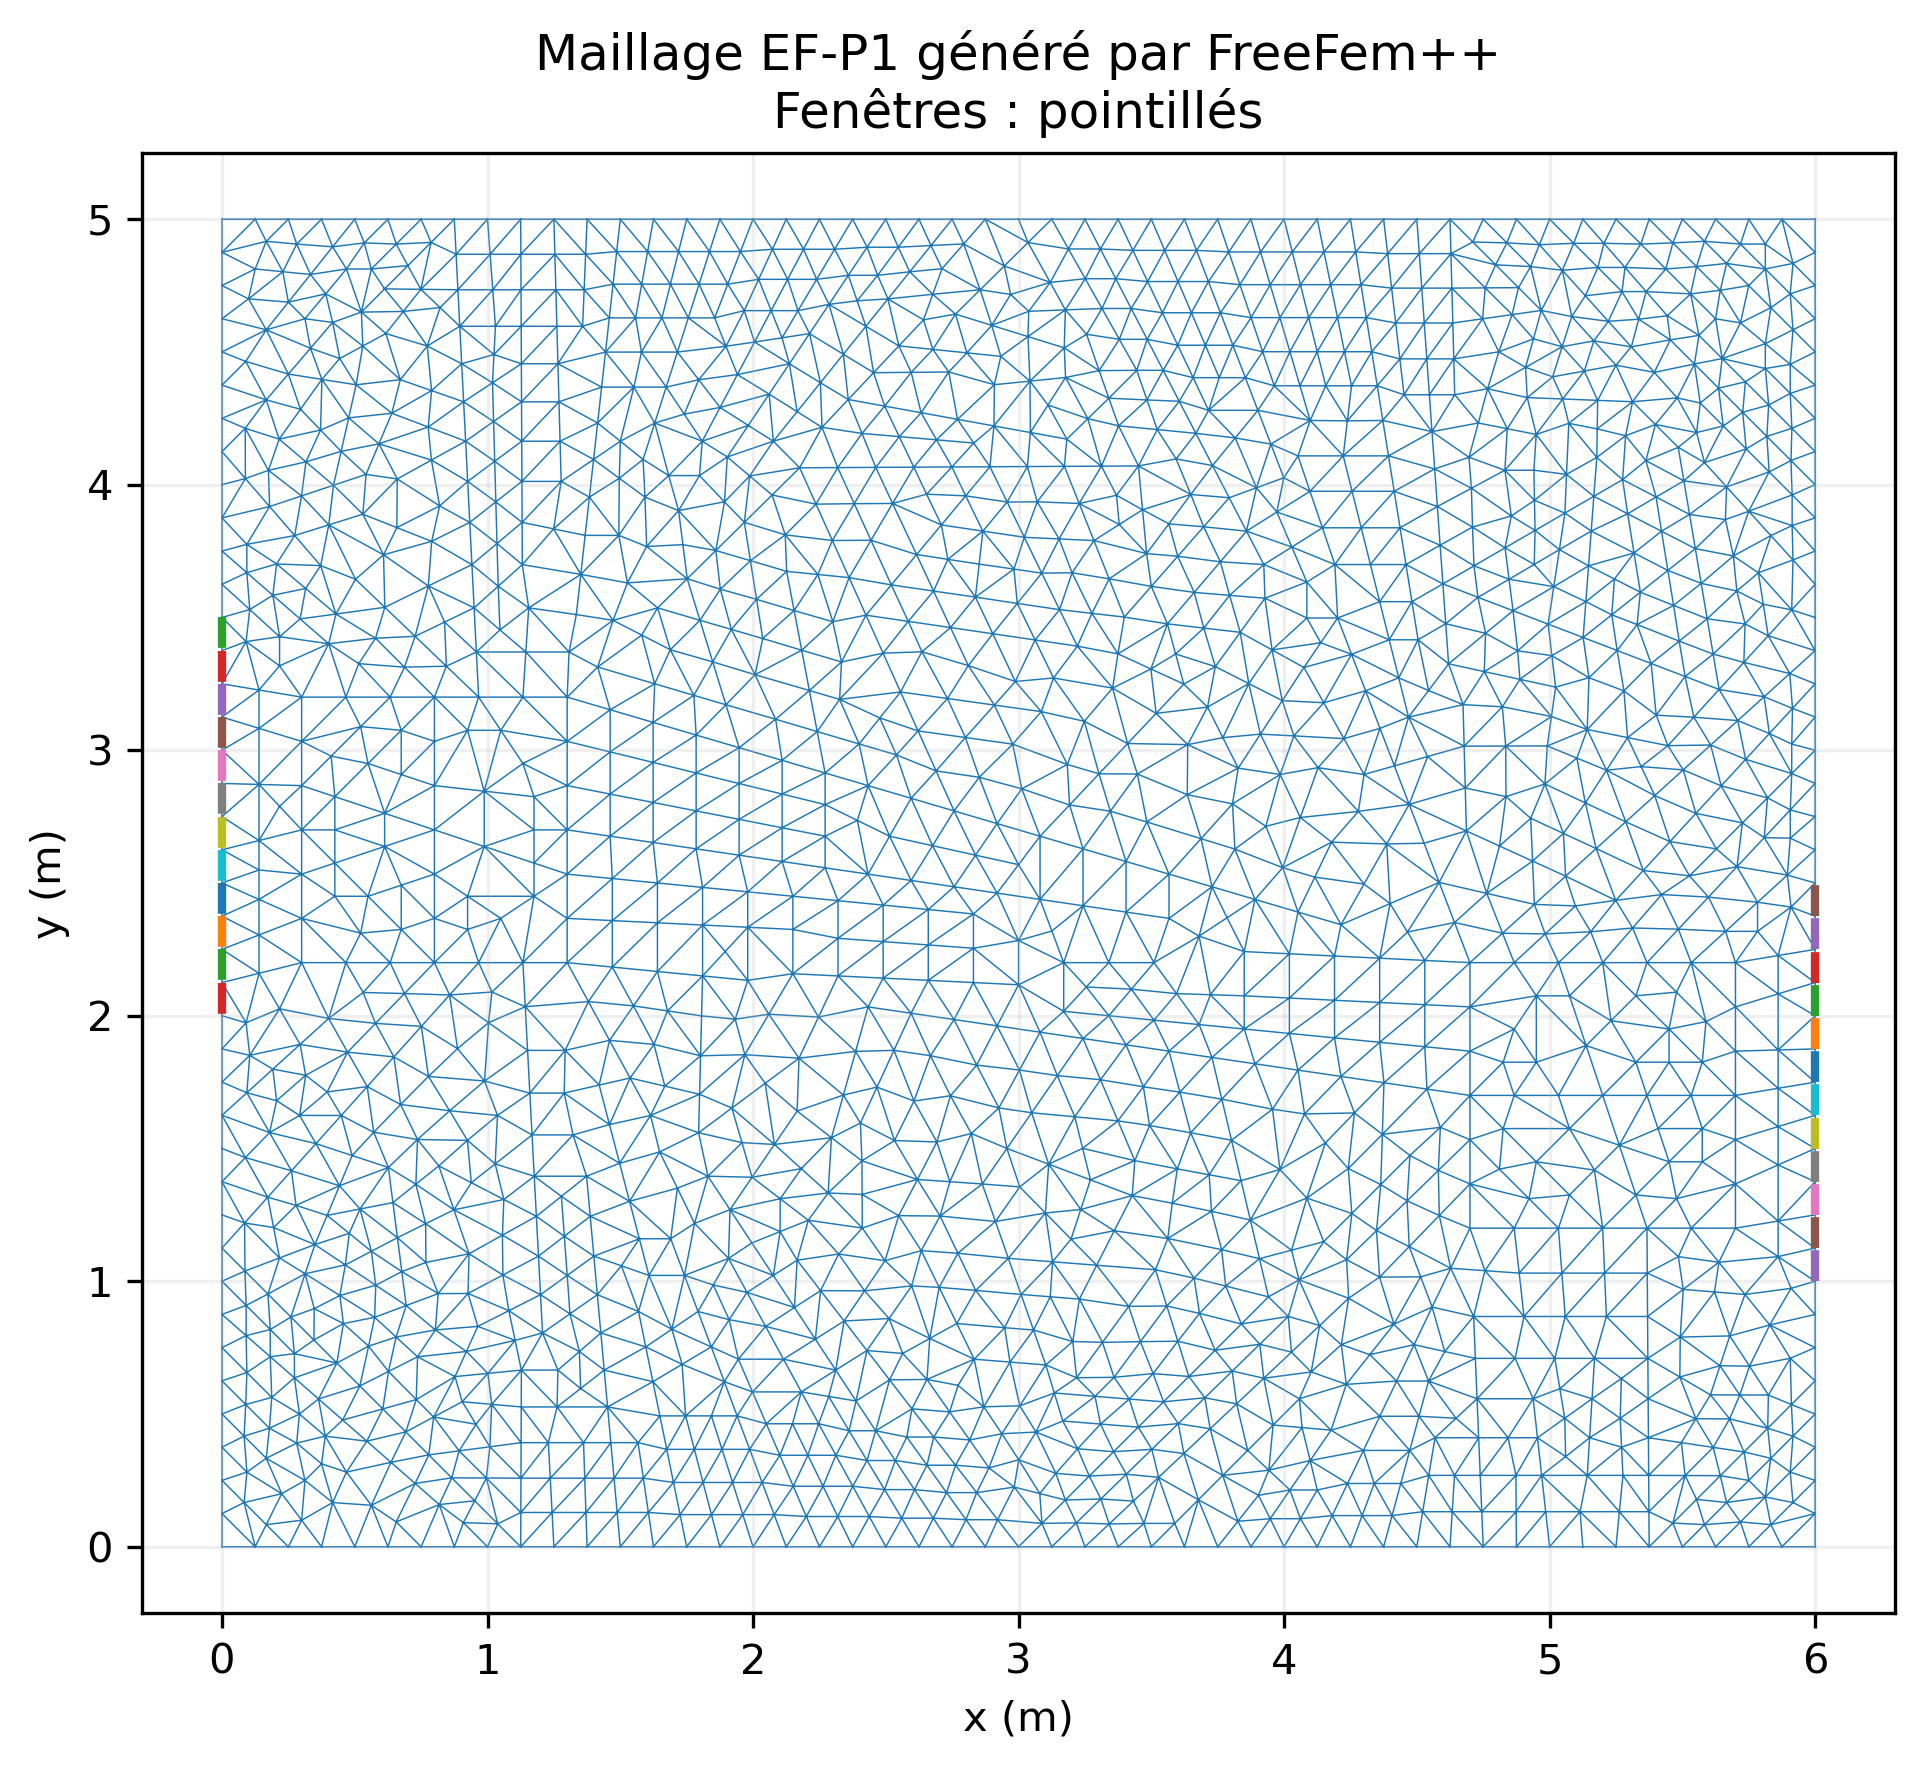
\includegraphics[width=0.72\textwidth]{figure5_maillage_EF_P1.png}
		\caption{Maillage triangulaire non structuré généré avec FreeFem++.}
		\label{fig:maillage-freefem}
	\end{figure}
	
	Ce maillage constitue le maillage de référence utilisé pour vérifier la
	cohérence de la géométrie et du modèle numérique.
	
	% -------------------------------------------------------------------------
	\section{Discrétisation par éléments finis P1}
	\label{sec:efp1}
	
	\subsection{Principe de la méthode des éléments finis}
	
	Après avoir construit le maillage du domaine $\Omega$, on cherche
	maintenant à approximer la solution du problème variationnel par une
	fonction définie sur ce maillage.
	
	Soit $\mathcal{T}_h$ le maillage triangulaire de $\Omega$. On note
	$N_s$ le nombre total de sommets et $N_t$ le nombre de triangles.
	
	On utilise des éléments finis de Lagrange de degré $1$, appelés
	éléments finis \textbf{P1}. Sur chaque triangle, l'approximation de la
	température est une fonction affine.
	
	\subsection{Fonctions de base P1}
	
	On introduit l'espace discret
	\[
	V_h =
	\left\{
	v_h\in\mathcal{C}^0(\overline{\Omega})
	:\;
	v_h|_K\in\mathbb{P}_1(K),
	\quad \forall K\in\mathcal{T}_h
	\right\}.
	\]
	
	Cet espace est engendré par les fonctions de base
	$(\varphi_i)_{i=1}^{N_s}$ vérifiant
	\[
	\varphi_i(S_j)=\delta_{ij}.
	\]
	Autrement dit, $\varphi_i$ est l'unique fonction affine par morceaux du maillage qui vaut $1$ au sommet $S_i$ et $0$ à tous les autres sommets. Ce choix n'est pas arbitraire : il rend l'interprétation du vecteur solution immédiate, comme le montre la remarque ci-dessous.
	
	La solution approchée s'écrit alors
	\[
	u_h(x,y)=\sum_{j=1}^{N_s}U_j\varphi_j(x,y),
	\]
	où $U_j$ représente la température au sommet $S_j$.
	
	\begin{quote}
		\small\emph{Remarque (pourquoi ce choix de base).} En évaluant $u_h$ au sommet $S_i$, la propriété $\varphi_j(S_i)=\delta_{ij}$ fait disparaître tous les termes de la somme sauf celui d'indice $j=i$ :
		\[
		u_h(S_i)=\sum_{j=1}^{N_s}U_j\,\varphi_j(S_i)=U_i.
		\]
		Le coefficient $U_i$ \emph{est} donc directement la température au nœud $i$ : aucune étape de décodage n'est nécessaire après résolution du système linéaire, le vecteur solution $U$ constitue déjà le champ de température nodal recherché.
	\end{quote}
	
	En remplaçant cette expression dans la formulation variationnelle et
	en choisissant successivement les fonctions tests $\varphi_i$, on
	obtient un système linéaire.
	
	\subsection{Matrice de rigidité locale}
	
	Considérons un triangle
	\[
	K=(S_1,S_2,S_3)
	\]
	de sommets
	\[
	S_i=(x_i,y_i).
	\]
	
	\begin{figure}[H]
		\centering
		\begin{tikzpicture}[scale=1.6, every node/.style={font=\small}]
			% Triangle générique K
			\coordinate (S1) at (0,0);
			\coordinate (S2) at (3,0.3);
			\coordinate (S3) at (0.8,2.2);
			\draw[very thick] (S1) -- (S2) -- (S3) -- cycle;
			
			\fill (S1) circle (1.5pt);
			\fill (S2) circle (1.5pt);
			\fill (S3) circle (1.5pt);
			\node[below left] at (S1) {$S_1=(x_1,y_1)$};
			\node[below right] at (S2) {$S_2=(x_2,y_2)$};
			\node[above] at (S3) {$S_3=(x_3,y_3)$};
			
			% Côté opposé à S1, en pointillé, pour illustrer b_1,c_1
			\draw[dashed, red!70!black, thick] (S2) -- (S3);
			\node[red!70!black, right] at ($(S2)!0.5!(S3)$) {\footnotesize côté opposé à $S_1$};
			
			% Petit label pour K et |K|
			\node at (1.2,0.8) {$K$};
			\node[align=left, font=\footnotesize] at (4.6,1.1)
			{$b_1=y_2-y_3$\\ $c_1=x_3-x_2$\\[4pt]
				$\nabla\varphi_1=\dfrac{1}{2|K|}(b_1,c_1)$\\[4pt]
				(perpendiculaire au côté\\ opposé à $S_1$)};
		\end{tikzpicture}
		\caption{Triangle générique $K$ du maillage. Le gradient $\nabla\varphi_1$ (constant sur $K$) est perpendiculaire au côté opposé au sommet $S_1$, et sa norme est inversement proportionnelle à l'aire $|K|$ : plus le triangle est petit, plus $\varphi_1$ doit croître rapidement pour passer de $0$ (sur le côté opposé) à $1$ (en $S_1$).}
		\label{fig:triangle-generique}
	\end{figure}
	
	Les gradients des fonctions de base P1 sont constants sur chaque
	triangle :
	\[
	\nabla\varphi_i
	=
	\frac{1}{2|K|}
	\begin{pmatrix}
		b_i\\
		c_i
	\end{pmatrix},
	\]
	avec
	\[
	\begin{aligned}
		b_1&=y_2-y_3,
		&
		b_2&=y_3-y_1,
		&
		b_3&=y_1-y_2,
		\\
		c_1&=x_3-x_2,
		&
		c_2&=x_1-x_3,
		&
		c_3&=x_2-x_1.
	\end{aligned}
	\]
	
	\begin{quote}
		\small\emph{Remarque (comment obtenir la formule de l'aire.)}
		\[
		|K|=\frac{1}{2}\big|(x_2-x_1)(y_3-y_1)-(x_3-x_1)(y_2-y_1)\big|,
		\]
		
		
		\emph{Vérification numérique.} Prenons le triangle simple $S_1=(0,0)$, $S_2=(1,0)$, $S_3=(0,1)$, d'aire $|K|=0{,}5$ (donc $2|K|=1$). L'unique fonction affine valant $1$ en $S_1$ et $0$ en $S_2,S_3$ est $\varphi_1(x,y)=1-x-y$, de gradient $\nabla\varphi_1=(-1,-1)$. Avec la formule : $b_1=y_2-y_3=-1$, $c_1=x_3-x_2=-1$, donc $\nabla\varphi_1=\frac{1}{1}(-1,-1)=(-1,-1)$ : les deux calculs coïncident exactement.
	\end{quote}
	
	La matrice de rigidité locale est donnée par
	\[
	(K_{\mathrm{loc}})_{ij}
	=
	\int_K
	\nabla\varphi_i\cdot\nabla\varphi_j\,dx
	=
	\frac{b_ib_j+c_ic_j}{4|K|}.
	\]
	
	\begin{quote}
		\small\emph{Remarque (comment on obtient cette formule).} Le gradient $\nabla\varphi_i$ étant \emph{constant} sur $K$, le produit scalaire $\nabla\varphi_i\cdot\nabla\varphi_j$ l'est aussi :
		\[
		\nabla\varphi_i\cdot\nabla\varphi_j=\frac{1}{2|K|}(b_i,c_i)\cdot\frac{1}{2|K|}(b_j,c_j)=\frac{b_ib_j+c_ic_j}{4|K|^2}.
		\]
		Intégrer une fonction \emph{constante} sur une région d'aire $|K|$ revient simplement à la multiplier par $|K|$ :
		\[
		\int_K \nabla\varphi_i\cdot\nabla\varphi_j\,dx = |K|\times\frac{b_ib_j+c_ic_j}{4|K|^2}=\frac{b_ib_j+c_ic_j}{4|K|}.
		\]
		Un seul des deux facteurs $|K|$ du dénominateur est simplifié par l'intégration ; c'est cette simplification qui rend le calcul exact et immédiat, sans recours à une intégration numérique -- une propriété propre aux éléments P1, dont le gradient est constant par morceaux.
	\end{quote}
	
	Comme le coefficient $\lambda$ est constant sur chaque région, la
	contribution réelle du triangle est
	\[
	K_{\mathrm{loc}}^{\lambda}
	=
	\lambda_K K_{\mathrm{loc}}.
	\]
	Le facteur géométrique $K_{\mathrm{loc}}$ (qui ne dépend que de la forme du triangle) et le facteur physique $\lambda_K$ (qui dépend de la région -- air ou radiateur) sont ainsi calculés séparément, ce qui permet de réutiliser la même géométrie de maillage pour des matériaux différents.
	
	\subsection{Vecteur local}
	
	Dans les radiateurs, la source $f$ est supposée constante par triangle.
	Le vecteur local est donc donné par
	\[
	(F_{\mathrm{loc}})_i
	=
	\int_K f_K\varphi_i\,dx.
	\]
	
	\begin{figure}[H]
		\centering
		\begin{tikzpicture}[scale=1.4, every node/.style={font=\small}]
			% Triangle de base K (aplati, aire = base)
			\coordinate (S1) at (0,0);
			\coordinate (S2) at (3,0.3);
			\coordinate (S3) at (0.8,2.2);
			\fill[gray!15] (S1) -- (S2) -- (S3) -- cycle;
			\draw[thick] (S1) -- (S2) -- (S3) -- cycle;
			\fill (S1) circle (1.5pt);
			\fill (S2) circle (1.5pt);
			\fill (S3) circle (1.5pt);
			\node[below left] at (S1) {$S_1$};
			\node[below right] at (S2) {$S_2$};
			\node[above right] at (S3) {$S_3$};
			\node at (1.3,0.85) {$K$ (aire $|K|$)};
			
			% Sommet de la "tente" au-dessus de S1, hauteur 1
			\coordinate (Apex) at ($(S1)+(0,2.8)$);
			\draw[dashed] (S1) -- (Apex) node[midway, left] {hauteur $=1$};
			\draw[very thick, blue!70!black] (Apex) -- (S2);
			\draw[very thick, blue!70!black] (Apex) -- (S3);
			\fill[blue!70!black] (Apex) circle (1.5pt);
			\node[above, blue!70!black] at (Apex) {$\varphi_1=1$};
			\node[align=left, right, font=\footnotesize] at (4.2,1.4) {Volume sous la tente\\$=\dfrac{1}{3}\times\text{base}\times\text{hauteur}=\dfrac{|K|}{3}$};
		\end{tikzpicture}
		\caption{Représentation en « tente » de la fonction de base $\varphi_1$ au-dessus du triangle $K$ : elle vaut $1$ au sommet $S_1$ et décroît linéairement jusqu'à $0$ sur le côté opposé $(S_2,S_3)$. L'intégrale $\int_K\varphi_1\,dx$ est exactement le volume sous cette tente, soit celui d'une pyramide de base $|K|$ et de hauteur $1$.}
		\label{fig:tente-phi}
	\end{figure}
	
	\begin{quote}
		
		\[
		\begin{aligned}
			\text{Volume}&=\frac{1}{3}\times\text{aire de la base}\times\text{hauteur}\\
			&=\frac{1}{3}\times|K|\times 1=\frac{|K|}{3}.
		\end{aligned}
		\]
		Ce résultat se retrouve aussi par intégration directe des coordonnées barycentriques (dont $\varphi_1$ est un exemple), à l'aide de la formule générale $\int_K\varphi_i^a\varphi_j^b\varphi_k^c\,dx=\frac{a!\,b!\,c!}{(a+b+c+2)!}\,2|K|$, qui donne bien $\frac{1}{6}\times2|K|=\frac{|K|}{3}$ pour $a=1,b=c=0$.
		
		\emph{Vérification numérique.} Sur le triangle de référence $S_1=(0,0)$, $S_2=(1,0)$, $S_3=(0,1)$ (aire $|K|=0{,}5$), on a $\varphi_1(x,y)=1-x-y$. Le calcul direct de l'intégrale double donne
		\[
		\int_K\varphi_1\,dx\,dy=\int_0^1\!\!\int_0^{1-x}(1-x-y)\,dy\,dx=\int_0^1\frac{(1-x)^2}{2}\,dx=\frac{1}{6},
		\]
		et la formule du rapport donne $|K|/3=0{,}5/3=1/6$ : les deux calculs coïncident exactement.
		
		\emph{Pourquoi les trois fonctions donnent la même intégrale.} Géométriquement, $\varphi_1,\varphi_2,\varphi_3$ sont trois tentes identiques, chacune pointant vers un sommet différent : aucune n'est privilégiée par la forme du triangle, donc les trois volumes sous ces tentes sont égaux. C'est pourquoi la formule $|K|/3$ est la même pour $i=1,2,3$.
	\end{quote}
	
	Or
	\[
	\int_K\varphi_i\,dx=\frac{|K|}{3},
	\]
	d'où
	\[
	(F_{\mathrm{loc}})_i
	=
	f_K\frac{|K|}{3},
	\qquad i=1,2,3.
	\]
	
	Cette formule admet une interprétation physique directe : le triangle génère au total une puissance $f_K\times|K|$, que l'on répartit \emph{équitablement} entre ses trois sommets, à raison d'un tiers chacun -- exactement ce que traduit la présence du facteur $\tfrac13$.
	
	Dans les triangles appartenant à l'air, on prend $f_K=0$ : ces triangles ne contribuent donc pas au second membre global, seuls les triangles situés à l'intérieur des radiateurs y ajoutent une contribution non nulle.
	
	\subsection{Assemblage global}
	
	Les matrices et vecteurs locaux calculés triangle par triangle (Sections~\ref{sec:efp1}.3 et \ref{sec:efp1}.4) ne portent que sur $3$ degrés de liberté à la fois. L'assemblage est l'opération qui les combine pour construire la matrice globale $K$ (de taille $N_s\times N_s$) et le vecteur global $F$ (de taille $N_s$), qui portent sur l'ensemble des $N_s$ sommets du maillage.
	
	Pour chaque triangle $K_e$, on note
	\[
	(I_1,I_2,I_3)
	\]
	les indices globaux de ses trois sommets.
	
	\begin{quote}
		\small\emph{Remarque (indices locaux et indices globaux).} À l'intérieur d'un triangle, les trois sommets sont numérotés $1,2,3$ (indices \emph{locaux}), tandis que dans le maillage complet, chaque sommet possède un numéro unique entre $1$ et $N_s$ (indice \emph{global}). Un même sommet local « $1$ » d'un triangle donné peut ainsi correspondre, par exemple, au sommet global numéro $847$ du maillage. Cette correspondance, stockée dans le tableau des indices $(I_1,I_2,I_3)$ de chaque triangle, indique \emph{où} placer chaque contribution locale dans la grande matrice.
	\end{quote}
	
	La contribution locale est alors ajoutée à la matrice globale selon
	\[
	K_{I_iI_j}
	\leftarrow
	K_{I_iI_j}
	+
	\lambda_e
	(K_{\mathrm{loc}})_{ij},
	\]
	et
	\[
	F_{I_i}
	\leftarrow
	F_{I_i}
	+
	(F_{\mathrm{loc}})_i.
	\]
	
	\begin{quote}
		\small\emph{Remarque (pourquoi accumuler plutôt qu'écrire).} La flèche $\leftarrow$ désigne une accumulation (« $\mathrel{+}=$ » en langage de programmation), et non une simple affectation. Cela est indispensable car un sommet global donné appartient généralement à \emph{plusieurs} triangles du maillage (plusieurs triangles du maillage). La fonction de base $\varphi_i$ associée à ce sommet est non nulle sur chacun de ces triangles, si bien que l'intégrale globale $\int_\Omega\lambda\nabla\varphi_i\cdot\nabla\varphi_j\,dx$ est en réalité la \emph{somme} des contributions de tous les triangles où $\varphi_i$ et $\varphi_j$ sont simultanément non nulles. Écraser la valeur au lieu de l'accumuler ferait perdre les contributions des triangles déjà traités.
	\end{quote}
	
	Cette opération est répétée pour tous les triangles du maillage. À l'issue de cette boucle, chaque entrée de $K$ et de $F$ contient exactement la somme de toutes les contributions locales pertinentes, conformément à la décomposition de l'intégrale sur $\Omega$ en somme d'intégrales sur chaque triangle.
	
	\subsection{Conditions de Dirichlet}
	
	Les conditions de Dirichlet sont imposées sur les sommets situés sur
	les fenêtres $\Gamma_D$ :
	\[
	u=u_D.
	\]
	
	Contrairement à la condition de Neumann homogène, qui est naturelle
	dans la formulation variationnelle (le terme de bord correspondant s'annule automatiquement, Section~\ref{sec:formulation-faible}), la condition de Dirichlet doit être
	imposée explicitement au niveau discret : elle contraint directement la valeur de $u$, ce qui ne peut pas « sortir » spontanément des équations variationnelles.
	
	On fixe donc les degrés de liberté correspondants à
	\[
	U_i=u_D.
	\]
	
	\begin{quote}
		\small\emph{Remarque (imposition numérique).} Dans l'implémentation finale, les degrés de liberté situés sur $\Gamma_D$ sont fixés directement à la valeur $u_D$. Les lignes et colonnes correspondantes sont prises en compte de manière à résoudre ensuite le système réduit sur les degrés de liberté libres. Cette méthode impose exactement la condition $U_i=u_D$ sans introduire de grand paramètre de pénalisation.
	\end{quote}
	
	\subsection{Système linéaire global}
	
	Après assemblage et prise en compte des conditions aux limites, le
	problème discret conduit au système linéaire
	\begin{equation}
		\label{eq:systeme}
		KU=F.
	\end{equation}
	
	\begin{quote}
		\small\emph{Remarque (d'où vient cette équation).} En substituant $u_h=\sum_j U_j\varphi_j$ dans la formulation variationnelle discrète $a(u_h,\varphi_i)=\ell(\varphi_i)$, héritière directe de \eqref{eq:variationnelle} (Section~\ref{sec:formulation-faible}), et en utilisant la bilinéarité de $a(\cdot,\cdot)$, on obtient, pour chaque $i$ :
		\[
		a(u_h,\varphi_i)=\sum_{j=1}^{N_s}U_j\,a(\varphi_j,\varphi_i)=\sum_{j=1}^{N_s}K_{ij}U_j.
		\]
		L'équation $a(u_h,\varphi_i)=\ell(\varphi_i)$ s'écrit donc $\sum_j K_{ij}U_j=F_i$ pour chaque $i$, ce qui est exactement la ligne $i$ du produit matrice-vecteur $KU=F$. Le passage de la formulation variationnelle discrète au système linéaire n'introduit donc aucune nouvelle hypothèse : c'est une simple réécriture matricielle compacte.
	\end{quote}
	
	où :
	\begin{itemize}
		\item $K$ est la matrice globale de rigidité ;
		\item $U$ est le vecteur des températures nodales ;
		\item $F$ est le vecteur global représentant les sources de chaleur (avant imposition de Dirichlet ; après cette étape, certaines de ses entrées codent en réalité la contrainte $M\,u_D$, cf. Section~\ref{sec:efp1}.6).
	\end{itemize}
	
	La résolution de ce système fournit les valeurs de la température aux
	différents sommets du maillage. Cette dernière étape relève de l'algèbre linéaire pure : une fois $K$ et $F$ fixés, plus aucune notion de triangle, de région ou de physique n'intervient, seule la structure creuse de la matrice importe pour la performance de la résolution.
	
	\subsection{Algorithme général}
	
	L'ensemble de la discrétisation peut être résumé par l'algorithme
	suivant.
	
	\begin{algorithm}[H]
		\caption{Assemblage du système EF-P1}
		\begin{algorithmic}[1]
			\State Entrée : maillage, $\lambda_1$, $\lambda_2$, $f_{\mathrm{rad}}$, $u_D$, $g$
			\State Initialiser $K$ et $F$
			\For{chaque triangle $K_e$}
			\State Calculer $|K_e|$
			\State Calculer les coefficients $b_i$ et $c_i$
			\State Calculer $K_{\mathrm{loc}}$
			\State Déterminer $\lambda_e$
			\State Ajouter $\lambda_e K_{\mathrm{loc}}$ dans $K$
			\State Calculer $F_{\mathrm{loc}}$
			\State Ajouter $F_{\mathrm{loc}}$ dans $F$
			\EndFor
			\State Repérer les noeuds de $\Gamma_D$
			\State Imposer $U_i=u_D$
			\State Ajouter la contribution de Neumann $g$ sur $\Gamma_N$
			\State Résoudre $KU=F$
			\State Retourner le champ de température $U$
		\end{algorithmic}
	\end{algorithm}
	
	Les formules précédentes constituent maintenant la base mathématique
	du solveur Python présenté dans la section suivante.
	
	% =========================================================================
	% =========================================================================
	\section{Implémentation Python}
	\label{sec:python}
	
	\subsection{Lecture directe du maillage FreeFem++}
	
	Le maillage de l'habitation est construit au préalable sous FreeFem++ à
	partir de la géométrie définie dans la Section~\ref{sec:maillage}. Il est
	ensuite exporté dans le fichier \texttt{habitation.mesh} à l'aide de la
	commande \texttt{savemesh}.
	
	Le programme Python ne reconstruit donc pas un nouveau maillage. Il lit
	directement le fichier \texttt{habitation.mesh} et récupère les coordonnées
	des noeuds, les triangles ainsi que les numéros de région et les labels des
	\textbf{arêtes de frontière}. Cette approche permet au solveur Python d'effectuer l'assemblage EF-P1
	à partir du maillage triangulaire généré par FreeFem++. Lorsque le même
	fichier de maillage est utilisé par les deux solveurs, la géométrie et la
	connectivité des éléments sont alors identiques.
	
	La chaîne de calcul utilisée est ainsi :
	\begin{center}
		\texttt{Géométrie $\rightarrow$ FreeFem++ $\rightarrow$ habitation.mesh
			$\rightarrow$ Python $\rightarrow$ assemblage EF-P1 $\rightarrow$ résolution.}
	\end{center}
	
	Les numéros de région sont attribués automatiquement par FreeFem++. Le
	programme Python ne suppose donc pas à l'avance qu'une région particulière
	correspond à l'air ou aux radiateurs. Il identifie l'air comme la région
	la plus représentée dans le maillage, puis considère les autres régions
	comme celles des radiateurs. Les labels des arêtes permettent notamment
	d'identifier les fenêtres portant le label 2, sur lesquelles la condition
	de Dirichlet est imposée.
	
	
	
	% -------------------------------------------------------------------------
	
	\subsection{Objectif de l'implémentation}
	
	La section précédente a permis d'établir les différentes formules
	nécessaires à la méthode des éléments finis P1.
	
	L'objectif de cette section est maintenant de traduire ces formules
	mathématiques en un programme Python capable de résoudre
	numériquement le problème de chauffage sur le maillage fourni par
	FreeFem++.
	
	Le solveur est développé \textbf{from scratch}, sans utiliser de
	bibliothèque spécialisée en éléments finis.
	
	Les principales étapes sont :
	\begin{enumerate}
		\item lire le maillage \texttt{habitation.mesh} produit par FreeFem++ ;
		\item récupérer les noeuds, les triangles, les régions et les labels de frontière ;
		\item calculer les matrices élémentaires P1 ;
		\item calculer les vecteurs locaux ;
		\item assembler la matrice globale et le second membre ;
		\item imposer les conditions de Dirichlet ;
		\item résoudre le système linéaire ;
		\item visualiser la solution obtenue.
	\end{enumerate}
	
	\subsection{Bibliothèques utilisées}
	
	L'implémentation repose principalement sur :
	\begin{itemize}
		\item \texttt{numpy} pour la manipulation des tableaux et les
		calculs numériques ;
		\item \texttt{scipy.sparse} pour la construction de la matrice
		creuse ;
		\item \texttt{scipy.sparse.linalg} pour la résolution du système
		linéaire ;
		\item \texttt{matplotlib} pour la visualisation du maillage et du
		champ de température.
	\end{itemize}
	
	\subsection{Lecture du fichier \texttt{habitation.mesh}}
	
	Le programme commence par vérifier la présence du fichier
	\texttt{habitation.mesh}. Il lit ensuite le bloc \texttt{Vertices} pour
	récupérer les coordonnées des sommets et le bloc \texttt{Triangles} pour
	récupérer la connectivité des éléments P1. Le numéro de région associé à
	chaque triangle est également conservé.
	
	Le bloc \texttt{Edges} est ensuite utilisé pour récupérer les arêtes de
	frontière et leurs labels. Les arêtes de label 2 correspondent aux
	fenêtres et permettent de déterminer directement les noeuds de
	\(\Gamma_D\).
	
	Ainsi, aucune reconstruction géométrique n'est nécessaire dans Python :
	les données géométriques et topologiques utilisées par le solveur sont
	celles du maillage FreeFem++.
	
	\subsection{Implémentation des formules P1}
	
	Pour chaque triangle, le programme récupère les coordonnées de ses trois
	sommets et calcule son aire.
	
	Il calcule ensuite les coefficients
	\[
	b_i,\qquad c_i,
	\]
	puis construit la matrice élémentaire selon la formule
	\[
	(K_{\mathrm{loc}})_{ij}
	=
	\frac{b_ib_j+c_ic_j}{4|K|}.
	\]
	
	La matrice est ensuite multipliée par le coefficient de conductivité thermique
	$\lambda_K$ correspondant à la région du triangle. Pour les radiateurs, le
	terme source $f_{\mathrm{rad}}$ est ajouté au second membre.
	
	\subsection{Assemblage de la matrice globale}
	
	Les contributions locales sont ajoutées dans la matrice globale $K$
	à partir des indices des trois sommets du triangle.
	
	Le principe informatique est directement issu de la formule
	mathématique :
	\[
	K_{I_iI_j}
	\leftarrow
	K_{I_iI_j}
	+
	\lambda_K(K_{\mathrm{loc}})_{ij}.
	\]
	
	Le second membre est assemblé simultanément :
	\[
	F_{I_i}
	\leftarrow
	F_{I_i}
	+
	(F_{\mathrm{loc}})_i.
	\]
	
	La matrice globale est stockée sous forme creuse afin de limiter la
	mémoire utilisée et d'accélérer la résolution.
	
	\subsection{Imposition de la condition de Dirichlet}
	
	Les noeuds situés sur les fenêtres sont identifiés à partir de leurs
	coordonnées.
	
	Pour chacun de ces noeuds, on impose
	\[
	U_i=u_D.
	\]
	
	Dans l'implémentation numérique finale, cette condition est imposée
	par une modification directe du système : les degrés de liberté associés
	aux noeuds de $\Gamma_D$ sont fixés à $u_D$, puis le système est résolu
	sur les degrés de liberté libres.
	
	\subsection{Résolution du système}
	
	Une fois l'assemblage terminé et les conditions de Dirichlet imposées,
	le programme résout le système
	\[
	KU=F.
	\]
	
	La résolution est réalisée avec
	\texttt{scipy.sparse.linalg.spsolve}.
	
	Le vecteur $U$ obtenu contient alors la température calculée à chaque
	noeud du maillage.
	
	\subsection{Visualisation des résultats}
	
	Une fois la résolution effectuée, le programme utilise
	\texttt{matplotlib} afin de représenter :
	\begin{itemize}
		\item le maillage triangulaire ;
		\item le champ de température ;
		\item une coupe unidimensionnelle de la température.
	\end{itemize}
	
	La Figure~\ref{fig:maillage} représente le maillage directement lu par
	Python depuis le fichier produit par FreeFem++.
	
	\begin{figure}[H]
		\centering
		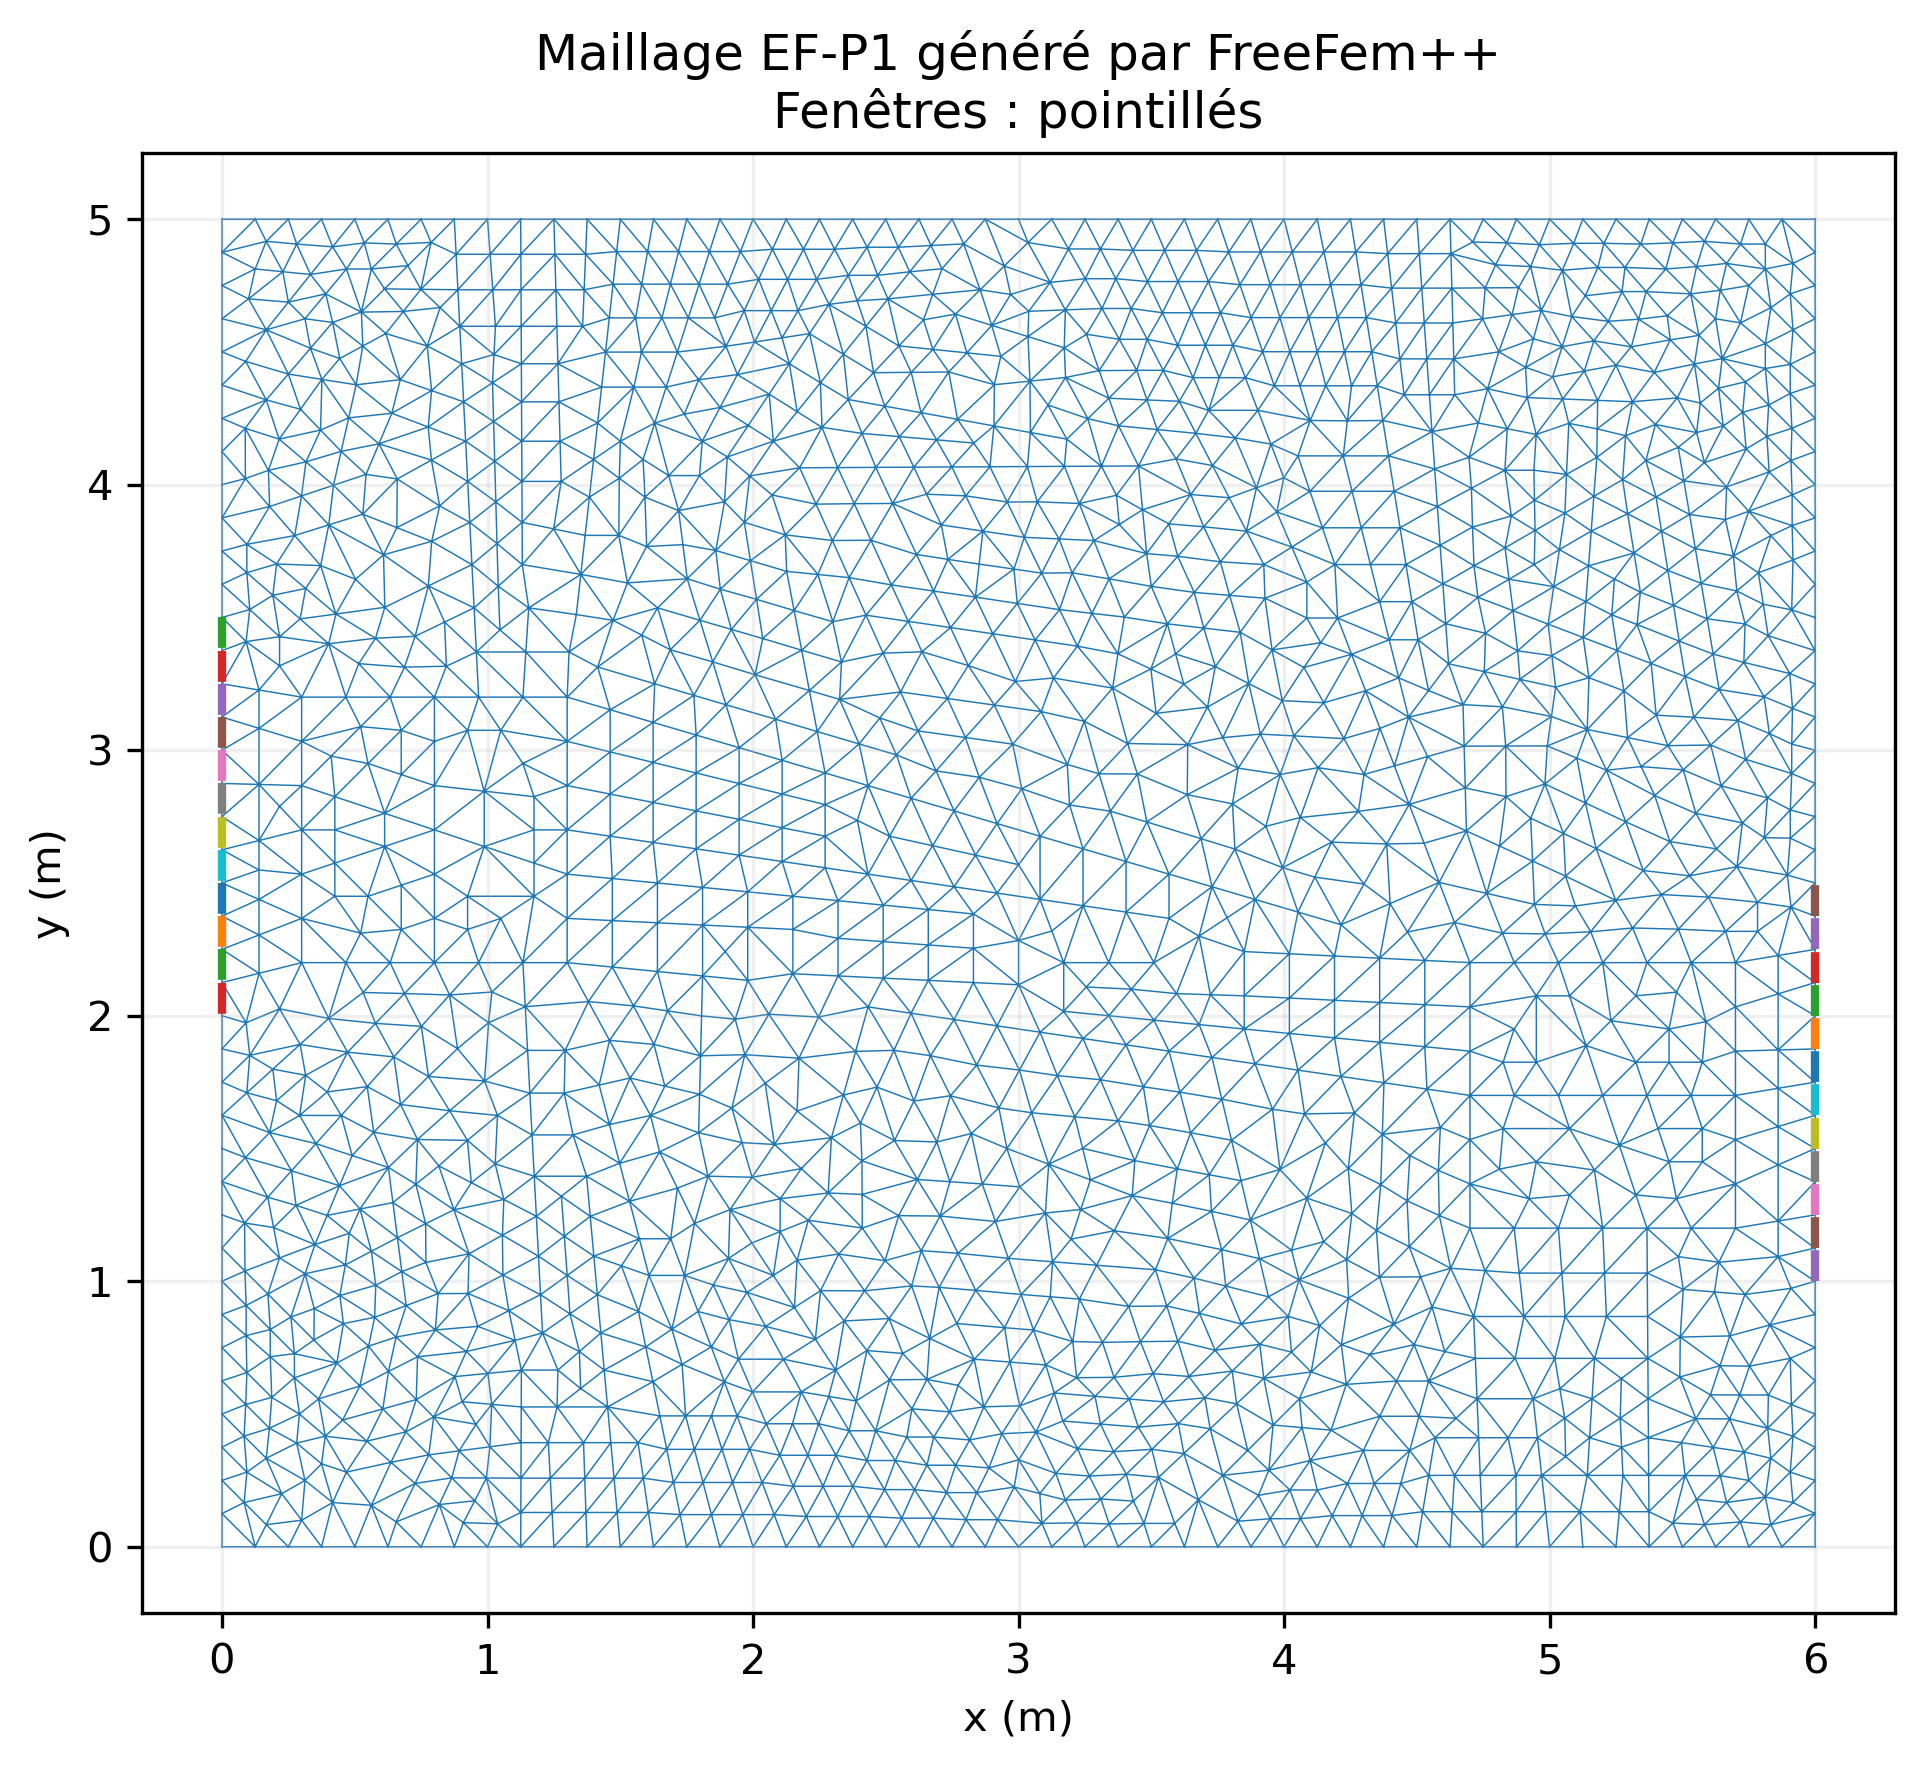
\includegraphics[width=0.72\textwidth]{figure5_maillage_EF_P1.png}
		\caption{Maillage EF-P1 généré par FreeFem++ et directement utilisé par Python.}
		\label{fig:maillage}
	\end{figure}
	\paragraph{Interprétation :}
	La Figure 5 présente le maillage triangulaire de l'habitation obtenu avec FreeFem++. On observe que le domaine est découpé en un ensemble de petits triangles qui constituent les éléments finis utilisés pour la résolution numérique. Les sommets de ces triangles représentent les degrés de liberté de l'approximation P1.
	
	Le maillage permet ainsi de représenter la géométrie de l'habitation et de distinguer les différentes régions du domaine, notamment la zone d'air et les zones correspondant aux radiateurs. Les frontières du domaine sont également conservées avec leurs labels afin de pouvoir identifier notamment les fenêtres et d'imposer les conditions aux limites.
	
	Ce maillage constitue donc la base de la méthode des éléments finis : le problème continu est discrétisé sur ces triangles avant l'assemblage de la matrice globale et du second membre.\\
	
	La Figure~\ref{fig:temperature} présente le champ de température stationnaire $u_h(x,y)$ obtenu par résolution du système \eqref{eq:systeme}.
	
	\begin{figure}[H]
		\centering
		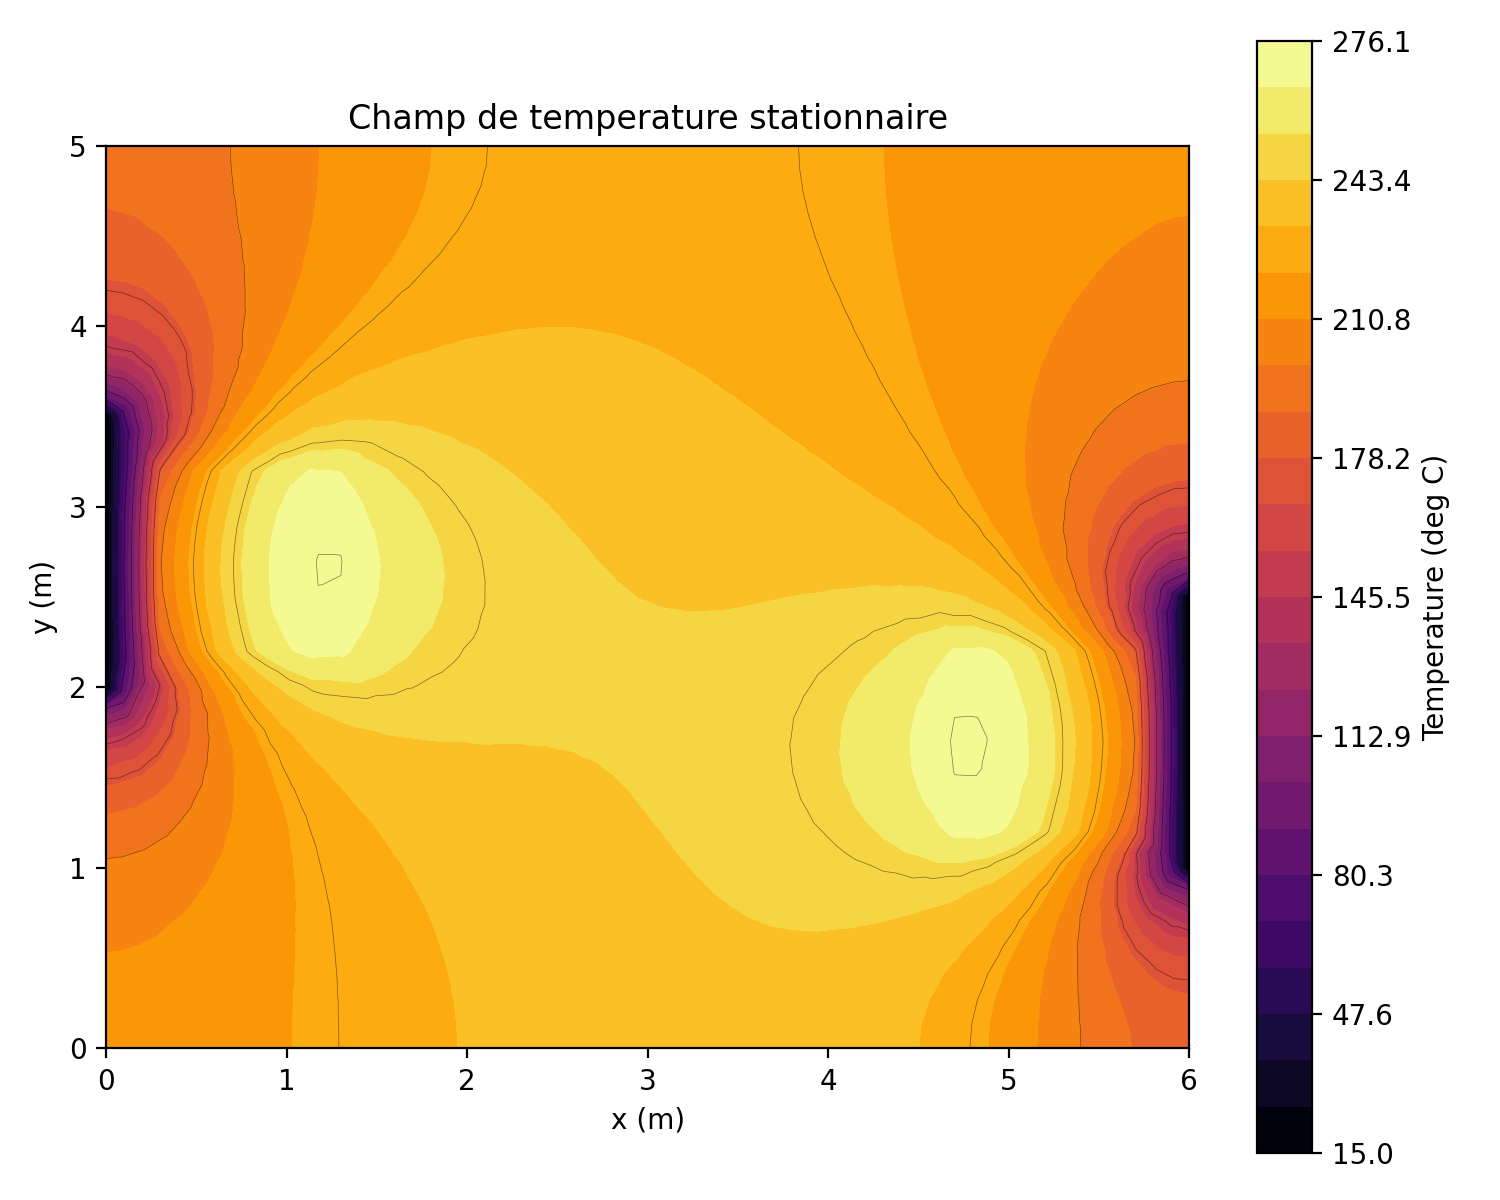
\includegraphics[width=0.75\textwidth]{temperature.png}
		\caption{Champ de température stationnaire $u_h(x,y)$ (en ${}^{\circ}$C) obtenu par le solveur EF-P1 Python. La fenêtre $F_2$ est soumise à la condition de Dirichlet $u=15\,{}^{\circ}$C.}
		\label{fig:temperature}
	\end{figure}
	\paragraph{Interprétation :}
	On observe que la température n'est pas uniforme dans l'habitation. Les températures les plus élevées se situent au voisinage des radiateurs, qui constituent les zones où la chaleur est produite. En s'éloignant des radiateurs, la température diminue progressivement sous l'effet de la diffusion thermique. On remarque également que la température atteint la valeur imposée de $15\,^\circ\mathrm{C}$ au niveau de la fenêtre soumise à la condition de Dirichlet. Cette figure permet donc de visualiser directement la diffusion de la chaleur dans les différentes zones de l'habitation.
	
	Pour mieux visualiser le gradient de température autour d'un radiateur, la Figure~\ref{fig:coupe1d} présente une coupe de la solution le long de la ligne horizontale $y=2.7$~m, qui traverse le radiateur R1 du salon.
	
	\begin{figure}[H]
		\centering
		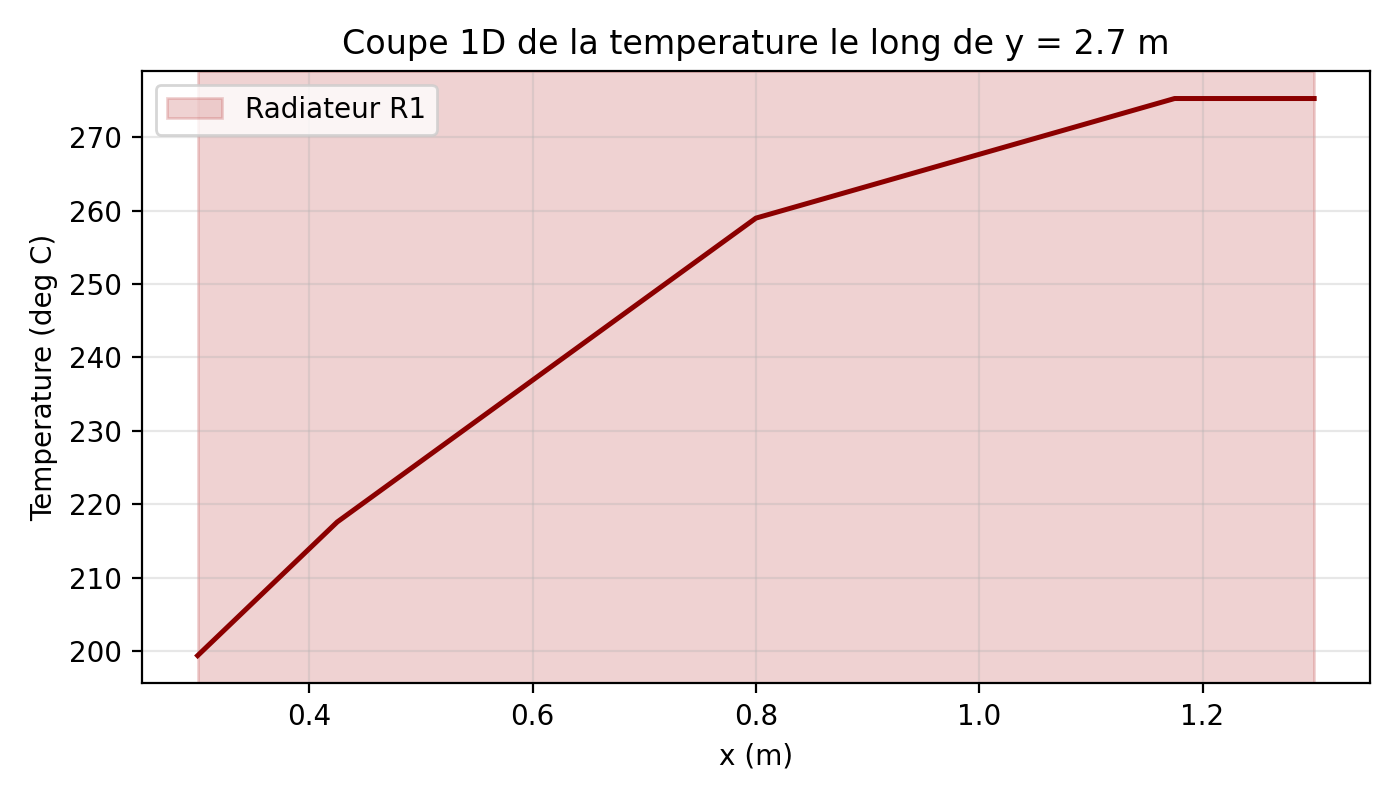
\includegraphics[width=0.8\textwidth]{coupe1d.png}
		\caption{Coupe 1D de la température le long de $y=2.7$~m, traversant le radiateur R1 (zone grisée).}
		\label{fig:coupe1d}
	\end{figure}
	\paragraph{Interprétation :}
	La coupe 1D permet d'observer plus précisément l'évolution de la température le long d'une ligne qui traverse le radiateur R1. On constate une augmentation importante de la température dans la zone du radiateur, puis une diminution progressive lorsqu'on s'en éloigne. Cela met en évidence le gradient de température créé par la source de chaleur. La coupe 1D complète donc la représentation 2D en permettant d'analyser l'évolution de la température suivant une direction donnée.
	
	Le champ numérique obtenu permet ainsi de visualiser les zones de forte
	température autour des radiateurs et l'influence des conditions imposées
	sur les fenêtres.
	
	
	\subsection{Cas de référence : condition de Neumann homogène}
	Le premier calcul numérique correspond au cas 1, avec $g=0$. Il constitue le problème de référence. Aucun terme de bord supplémentaire n'est assemblé pour la condition de Neumann homogène.
	
	\subsection{Influence de la puissance des radiateurs}
	
	L'étape 4 consiste à étudier l'influence de la puissance volumique
	$f_{\mathrm{rad}}$ des radiateurs sur la température calculée. Les
	paramètres imposés sont
	\[
	\lambda_{\mathrm{air}}=0{,}25,\qquad
	\lambda_{\mathrm{rad}}=1,\qquad
	u_D=15.
	\]
	Les valeurs
	\[
	f_{\mathrm{rad}}\in\{0,50,100,150,200,250\}
	\]
	sont testées successivement avec les deux radiateurs en fonctionnement.
	
	Pour chaque valeur, le programme assemble la matrice de rigidité et le
	second membre, impose la condition de Dirichlet sur les fenêtres, puis
	calcule les températures minimale, maximale et moyenne.
	
	Les résultats obtenus sont présentés dans le tableau suivant.
	
	\begin{table}[H]
		\centering
		\caption{Influence de la puissance volumique des radiateurs}
		\begin{tabular}{c|ccc}
			\hline
			$f_{\mathrm{rad}}$ (W/m$^3$) & $T_{\min}$ (\textdegree C) & $T_{\max}$ (\textdegree C) & $T_{\mathrm{moy}}$ (\textdegree C) \\
			\hline
			0   & 15.000 & 15.000 & 15.000 \\
			50  & 15.000 & 67.217 & 56.798 \\
			100 & 15.000 & 119.434 & 98.597 \\
			150 & 15.000 & 171.651 & 140.395 \\
			200 & 15.000 & 223.868 & 182.194 \\
			250 & 15.000 & 276.085 & 223.992 \\
			\hline
		\end{tabular}
	\end{table}
	
	Les valeurs du tableau sont celles obtenues avec le maillage
	\texttt{habitation.mesh} comportant 1756 nœuds et 3334 triangles.
	La température moyenne est calculée comme une moyenne intégrale pondérée
	par l'aire des éléments, et non comme une simple moyenne des valeurs nodales.
	
	
	On constate que l'augmentation de la puissance volumique des radiateurs
	entraîne une augmentation régulière de la température maximale et de la
	température moyenne. La température minimale reste égale à $15\,{}^\circ\mathrm{C}$
	en raison de la condition de Dirichlet imposée sur la fenêtre $F_2$.
	
	La Figure~\ref{fig:etape4_puissance} présente l'influence de la puissance
	volumique des radiateurs sur les températures calculées.
	
	\begin{figure}[H]
		\centering
		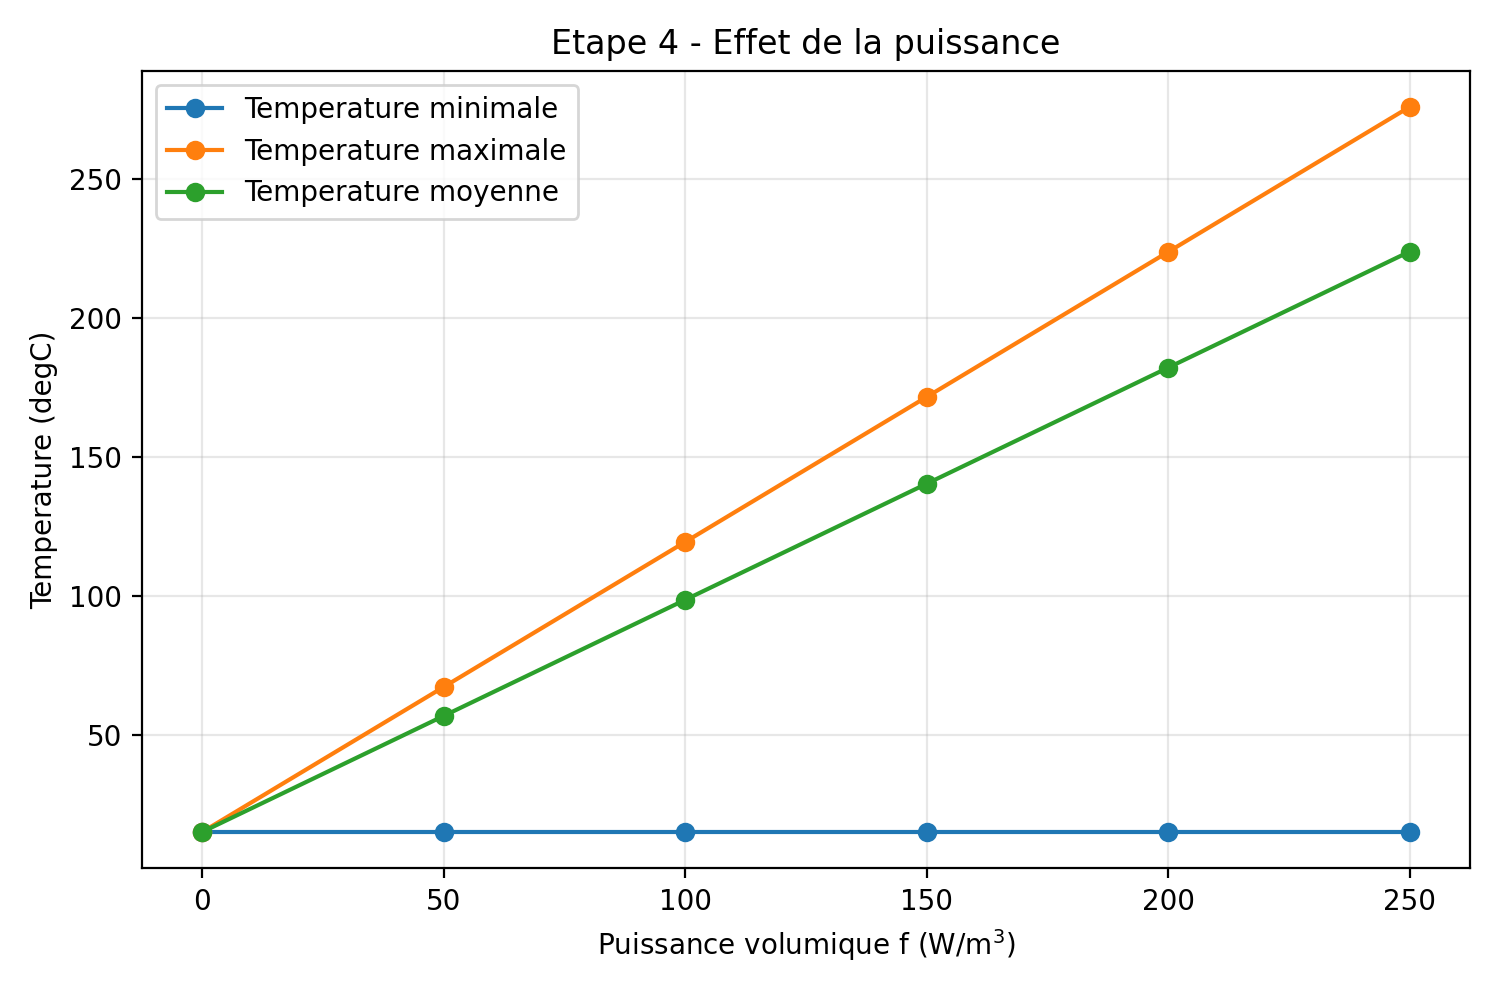
\includegraphics[width=0.85\textwidth]{etape4_puissance.png}
		\caption{Influence de la puissance volumique des radiateurs sur la température.}
		\label{fig:etape4_puissance}
	\end{figure}
	\paragraph{Interprétation :}
	Cette figure montre clairement l'influence de la puissance volumique des radiateurs sur la température dans l'habitation. Lorsque la puissance $f_{\mathrm{rad}}$ augmente, la température maximale et la température moyenne augmentent également de manière régulière. Cela s'explique par le fait qu'une puissance plus importante correspond à une production de chaleur plus importante dans les zones occupées par les radiateurs.
	
	La température minimale reste égale à $15\,^\circ\mathrm{C}$, car cette température est imposée sur la fenêtre par la condition de Dirichlet. La puissance des radiateurs agit donc principalement sur les températures maximale et moyenne, tandis que la température minimale est fixée par la condition aux limites.
	
	La Figure~\ref{fig:etape4_allumage} compare les différentes configurations
	d'allumage des radiateurs pour $f_{\mathrm{rad}}=250$.
	
	\begin{figure}[H]
		\centering
		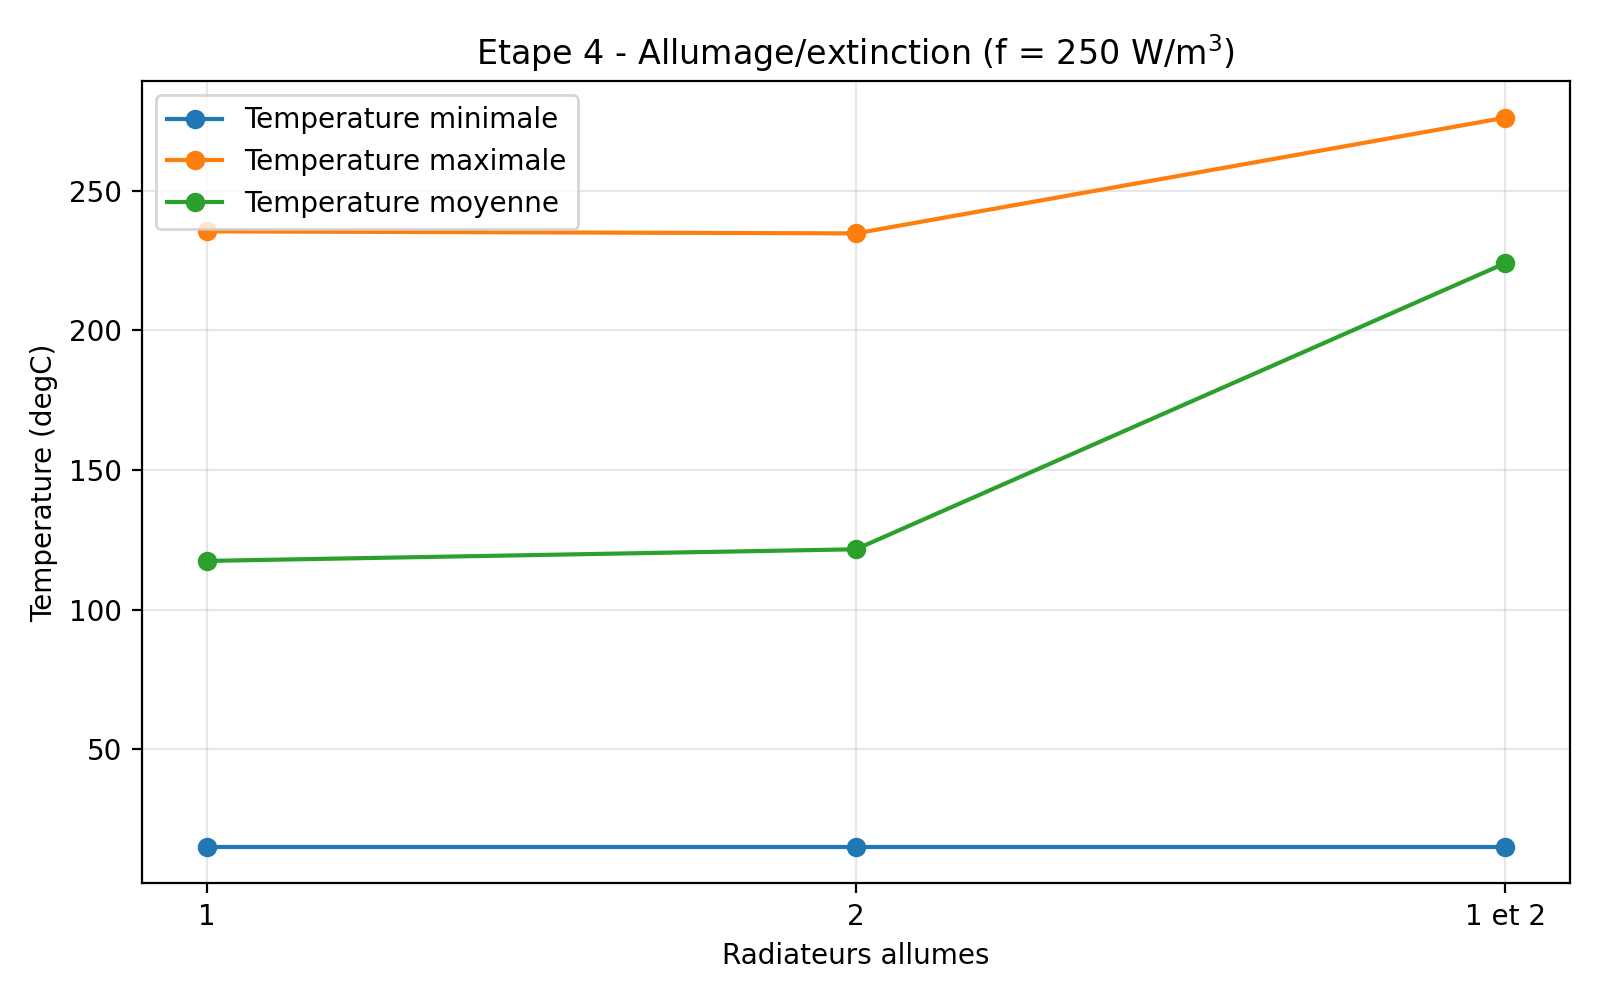
\includegraphics[width=0.85\textwidth]{etape4_allumage.png}
		\caption{Comparaison des différentes configurations d'allumage des radiateurs.}
		\label{fig:etape4_allumage}
	\end{figure}
	\paragraph{Interprétation :}
	Cette figure permet d'étudier l'influence de la configuration d'allumage des radiateurs. Lorsqu'un seul radiateur fonctionne, l'augmentation de température est principalement localisée autour de celui-ci. Lorsque les deux radiateurs fonctionnent simultanément, les deux sources de chaleur contribuent au chauffage de l'habitation. On obtient alors une température moyenne et une température maximale plus importantes.
	
	On constate donc que la répartition des sources de chaleur dans l'habitation influence directement la distribution de la température.
	
	Les résultats obtenus pour les différentes configurations sont :
	\begin{center}
		\begin{tabular}{l|ccc}
			\hline
			Configuration & $T_{\min}$ (\textdegree C) & $T_{\max}$ (\textdegree C) & $T_{\mathrm{moy}}$ (\textdegree C) \\
			\hline
			Radiateur 1 seul & 15.000 & 235.399 & 117.414 \\
			Radiateur 2 seul & 15.000 & 234.676 & 121.578 \\
			Radiateurs 1 et 2 & 15.000 & 275.085 & 223.992 \\
			\hline
		\end{tabular}
	\end{center}
	
	Cette comparaison montre que le fonctionnement simultané des deux
	radiateurs produit la température moyenne la plus élevée.
	
	\subsection{Condition de Neumann non homogène}
	\label{sec:etape5}
	
	Dans cette étude, la condition de Neumann homogène est remplacée sur $F_1$
	par une condition de Neumann non homogène de la forme
	\[
	-\lambda \frac{\partial u}{\partial n}=g(x),
	\]
	où $g(x)\geq 0$ représente le flux thermique imposé sur la frontière.
	
	Dans notre étude, on considère un flux constant
	\[
	g=5.
	\]
	
	Une partie de la frontière est soumise à cette condition de Neumann
	non homogène, tandis qu'au moins une fenêtre reste soumise à une
	condition de Dirichlet afin d'assurer l'unicité de la solution.
	
	\subsubsection{Formulation variationnelle}
	
	La condition de Neumann non homogène introduit un terme supplémentaire
	dans le second membre de la formulation variationnelle :
	\[
	\int_{\Gamma_N} g\,v\,d\sigma.
	\]
	
	Ce terme doit être calculé numériquement lors de l'assemblage du système
	d'éléments finis.
	
	\subsubsection{Quadrature numérique 1D du terme de bord}
	\label{sec:quadrature-1d}
	
	
	Le terme de bord associé à la condition de Neumann non homogène est
	\[
	\int_{\Gamma_N} g\,v\,d\sigma.
	\]
	Pour son calcul numérique, on décompose $\Gamma_N$ en arêtes du maillage.
	Considérons une arête $e=[P_i,P_j]$ de longueur $\ell_e$. Avec des éléments
	finis P1, la fonction test est affine sur cette arête et ses fonctions de base
	locales vérifient
	\[
	\varphi_i(P_i)=1,\qquad \varphi_i(P_j)=0,\qquad
	\varphi_j(P_i)=0,\qquad \varphi_j(P_j)=1.
	\]
	
	Dans notre problème, le flux imposé est constant, $g=5$. La règle du trapèze
	en dimension 1 donne alors
	\[
	\int_e g\,\varphi_i\,d\sigma
	\simeq \frac{\ell_e}{2}\bigl(g\varphi_i(P_i)+g\varphi_i(P_j)\bigr)
	= \frac{g\ell_e}{2},
	\]
	et de même
	\[
	\int_e g\,\varphi_j\,d\sigma = \frac{g\ell_e}{2}.
	\]
	Ainsi, chaque arête de frontière portant le flux $g$ apporte la contribution
	$g\ell_e/2$ à chacun de ses deux nœuds. Comme $g$ est constant et que les
	fonctions de base P1 sont affines sur chaque arête, cette quadrature est exacte
	dans le cas considéré. Le vecteur de bord est ensuite obtenu en additionnant
	les contributions de toutes les arêtes de $F_1$.
	
	
	Cette quadrature permet d'assembler numériquement le vecteur associé au
	terme de Neumann non homogène. Dans notre cas, elle est appliquée sur les
	arêtes de $F_1$ portant le flux constant $g=5$.
	
	\subsubsection{Résolution numérique}
	
	Le vecteur de bord est assemblé en additionnant les contributions $g\ell_e/2$
	sur les arêtes de $F_1$. Avec la convention $-\lambda\partial_n u=g$,
	cette contribution est prise en compte avec le signe correspondant dans le
	système discret. La condition de Dirichlet est ensuite imposée exactement
	sur $F_2$, puis le système creux est résolu numériquement avec Python.
	
	Les résultats numériques obtenus pour l'étape 5 sont présentés dans le
	tableau~\ref{tab:resultats-etape5}.
	
	\begin{table}[H]
		\centering
		\begin{tabular}{lc}
			\hline
			\textbf{Grandeur} & \textbf{Valeur} \\
			\hline
			Nombre de nœuds & 1756 \\
			Nombre de triangles & 3334 \\
			Température minimale & $15.000000\,{}^\circ\mathrm{C}$ \\
			Température maximale & $275.509108\,{}^\circ\mathrm{C}$ \\
			Température moyenne & $183.623546\,{}^\circ\mathrm{C}$ \\
			\hline
		\end{tabular}
		\caption{Résultats numériques de l'étape 5.}
		\label{tab:resultats-etape5}
	\end{table}
	
	Le calcul est effectué sur le maillage \texttt{habitation\_etape5.mesh},
	qui comporte 1756 nœuds et 3334 triangles. Le champ de température obtenu
	est présenté à la Figure~\ref{fig:etape5_temperature}.
	
	\begin{figure}[H]
		\centering
		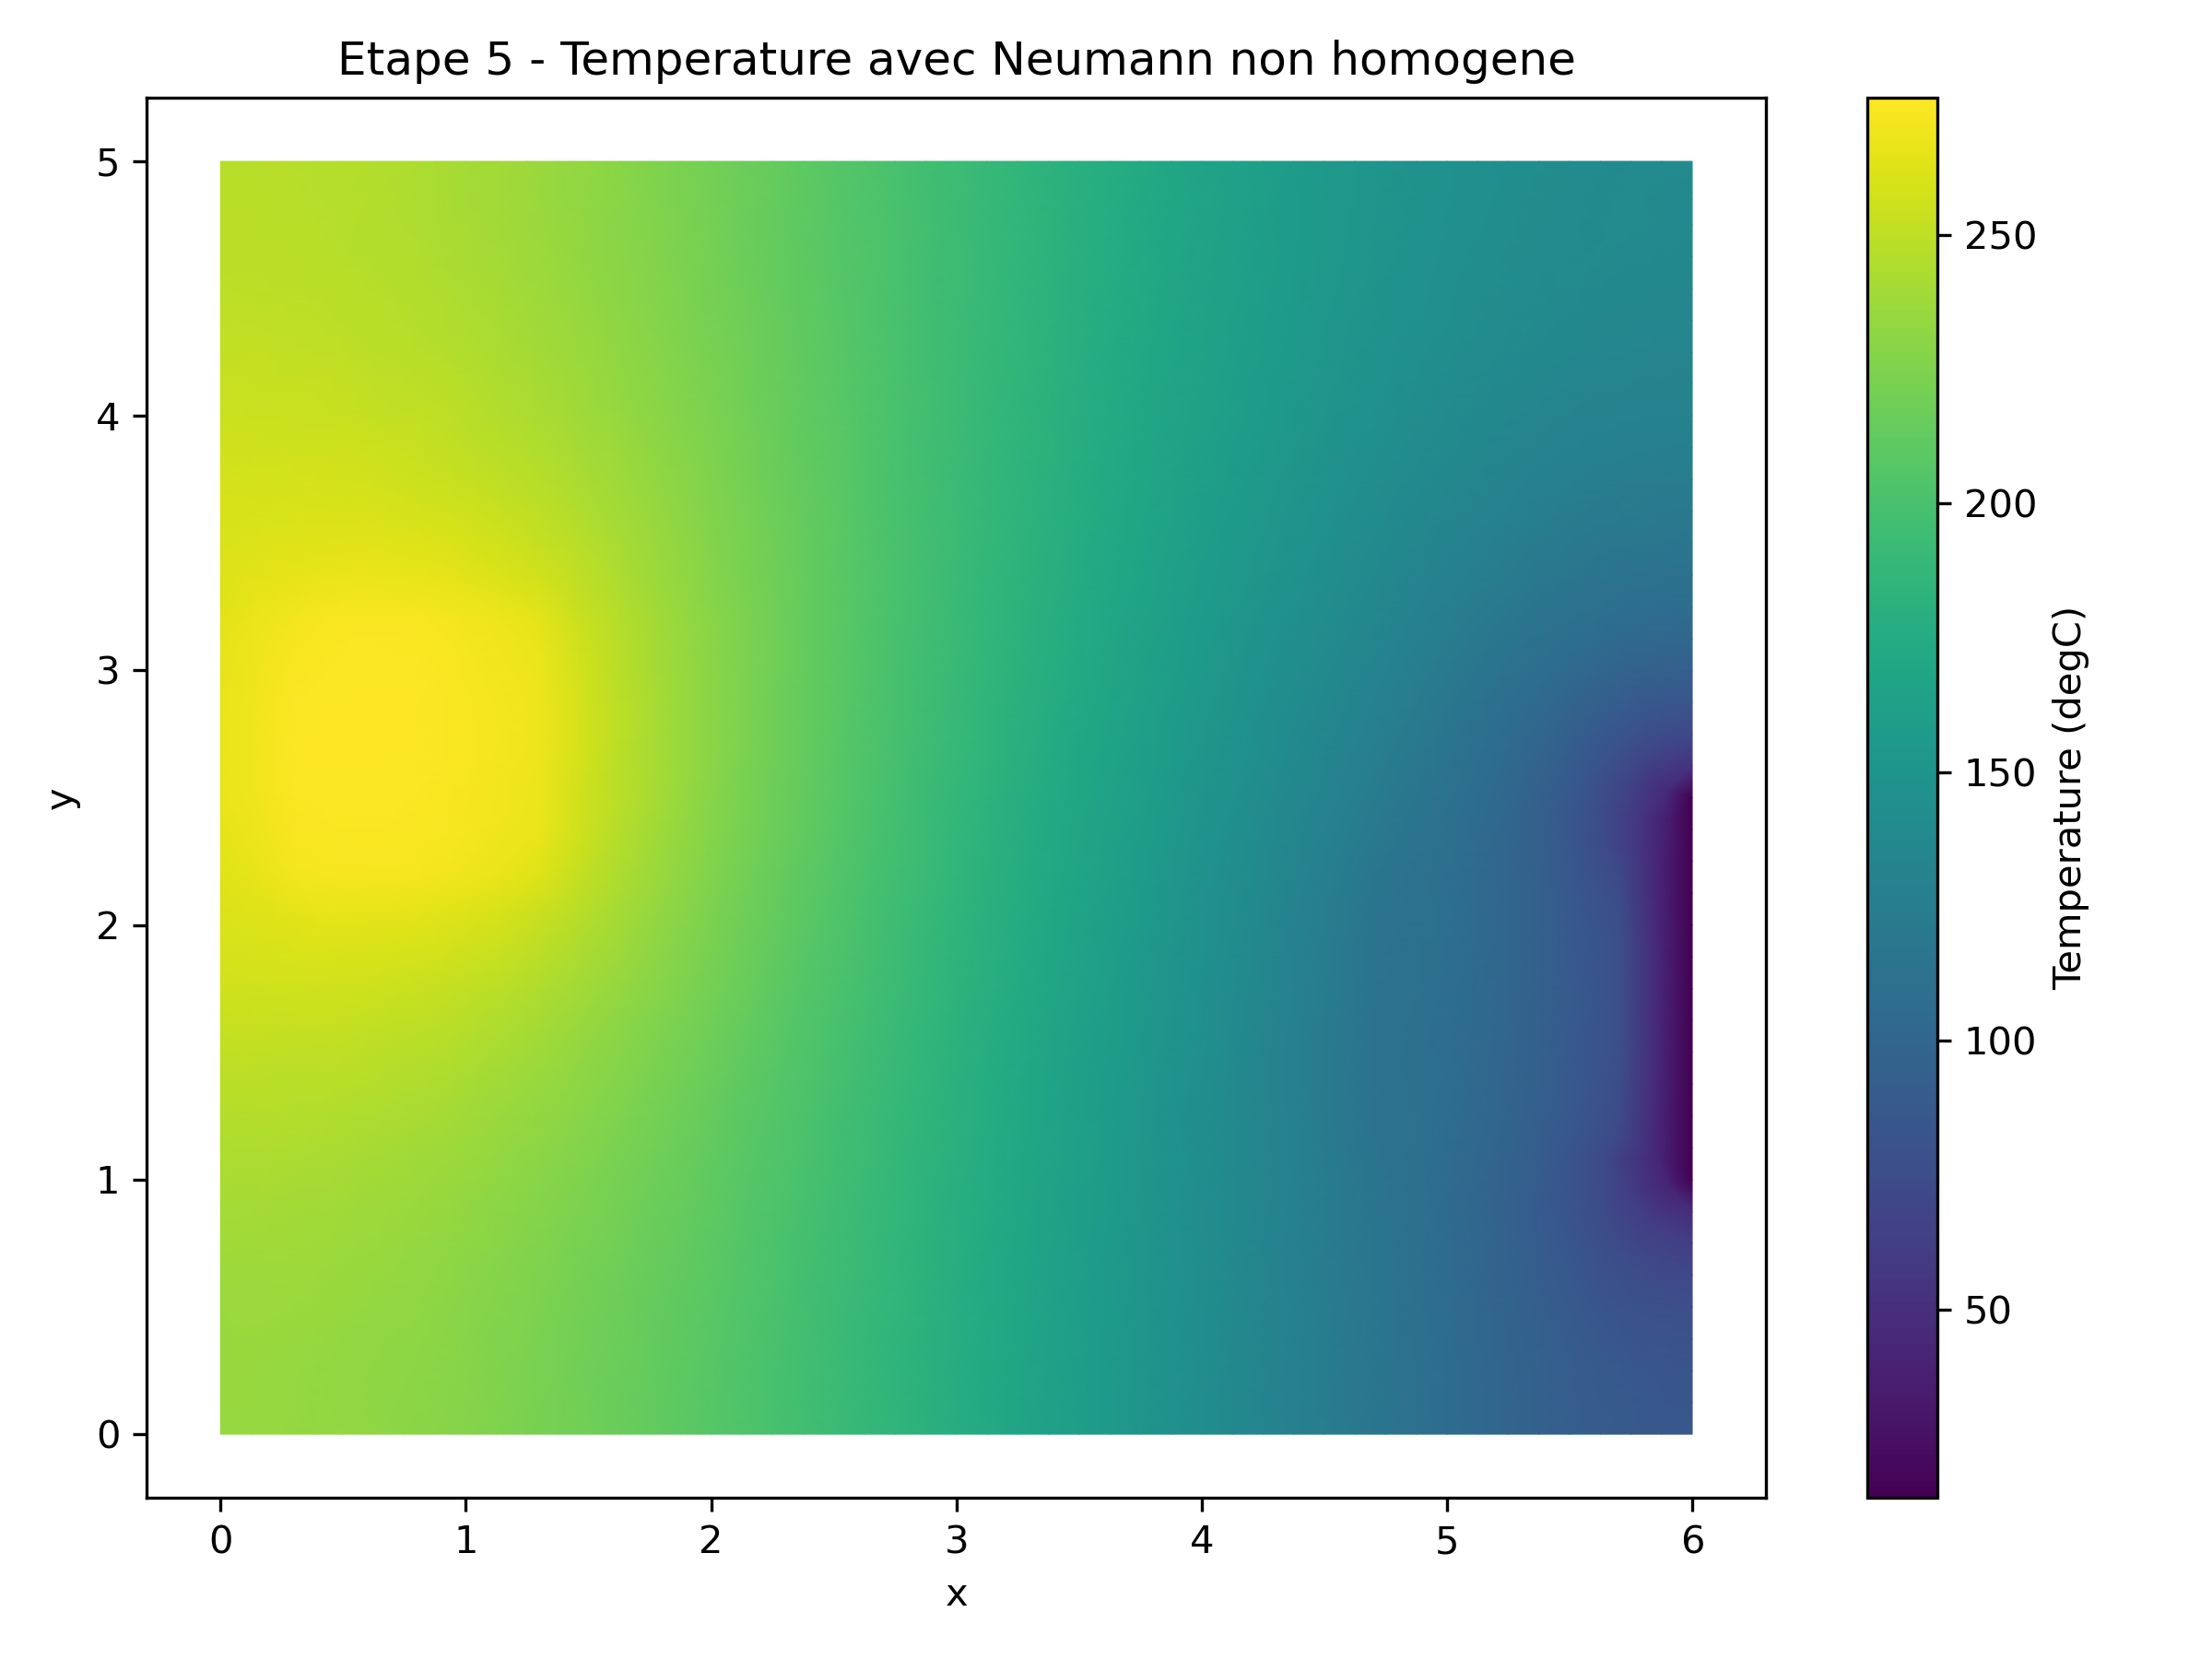
\includegraphics[width=0.85\textwidth]{../etape5_temperature.png}
		\caption{Champ de température obtenu avec une condition de Neumann non homogène.}
		\label{fig:etape5_temperature}
	\end{figure}
	
	\paragraph{Interprétation}
	La Figure 10 présente le champ de température obtenu après l'introduction d'une condition de Neumann non homogène sur une partie de la frontière. On observe que la température est influencée à la fois par les sources de chaleur présentes dans l'habitation et par le flux thermique imposé sur cette frontière. La température reste fixée à $15\,^\circ\mathrm{C}$ sur la fenêtre soumise à la condition de Dirichlet, tandis qu'un flux thermique est imposé sur la frontière soumise à la condition de Neumann. Cette modification permet ainsi de représenter une situation où un échange thermique est présent à travers la frontière.
	
	\subsection{Vérification par un solveur équivalent en FreeFem++}
	
	Conformément à l'\textbf{Option 3} proposée dans le sujet, le même
	problème mathématique que celui de l'étape 5 est résolu directement avec
	FreeFem++. L'objectif est de disposer d'un solveur équivalent et de comparer
	les résultats obtenus avec ceux du solveur Python. Les paramètres utilisés
	sont
	\[
	\lambda_{\mathrm{air}}=0{,}25,\qquad
	\lambda_{\mathrm{rad}}=1,\qquad
	f_{\mathrm{rad}}=50,\qquad
	u_D=15,\qquad g=5.
	\]
	
	Le programme FreeFem++ utilise directement les régions détectées dans le
	maillage pour conserver les coefficients constants par élément. La source
	est intégrée uniquement dans les deux régions des radiateurs et la condition
	de Neumann non homogène est imposée sur le label correspondant à $F_1$.
	
	Les deux solveurs utilisent le même fichier de maillage
	\texttt{habitation\_etape5.mesh}, comportant 1756 nœuds et 3334 triangles.
	Les paramètres physiques sont également identiques :
	\[
	\lambda_{\mathrm{air}}=0{,}25,\qquad
	\lambda_{\mathrm{rad}}=1,\qquad
	f_{\mathrm{rad}}=50,\qquad
	u_D=15,\qquad g=5.
	\]
	
	Le solveur Python de l'étape 5 donne :
	\[
	T_{\min}=15.000000\,{}^\circ\mathrm{C},\qquad
	T_{\max}=275.509108\,{}^\circ\mathrm{C},
	\]
	\[
	T_{\mathrm{moy}}=183.623546\,{}^\circ\mathrm{C}.
	\]
	
	Le solveur FreeFem++ de l'étape 6 donne, à l'arrondi affiché :
	\[
	T_{\min}=15.000\,{}^\circ\mathrm{C},\qquad
	T_{\max}=275.000\,{}^\circ\mathrm{C},
	\]
	\[
	T_{\mathrm{moy}}=183.624\,{}^\circ\mathrm{C}.
	\]
	
	Les deux calculs utilisent donc le même maillage et les mêmes paramètres.
	Les valeurs obtenues sont concordantes, ce qui permet de vérifier la
	cohérence de l'implémentation Python par une seconde résolution indépendante
	avec FreeFem++.
	
	\begin{figure}[H]
		\centering
		\IfFileExists{../figures/etape6_temperature_freefem.png}{\includegraphics[width=0.85\textwidth]{../figures/etape6_temperature_freefem.png}}{\fbox{\parbox{0.8\textwidth}{\centering Figure non disponible dans le dossier figures du dépôt.}}}
		\caption{Distribution de la température obtenue avec FreeFem++ à l'étape 6.}
		\label{fig:etape6_freefem}
	\end{figure}
	\paragraph{Interprétation de la Figure 11.}
	La Figure 11 présente la distribution de la température obtenue avec
	FreeFem++ à l'étape 6. Cette simulation reprend le même problème
	physique que celui considéré à l'étape 5, avec une condition de
	Neumann non homogène sur une partie de la frontière. La distribution
	obtenue est qualitativement proche de celle calculée avec le solveur
	Python à l'étape 5. Les éventuelles différences dans la représentation
	des isothermes s'expliquent notamment par les différences de maillage
	et de visualisation entre les deux implémentations. Cette comparaison
	constitue ainsi une vérification de cohérence du solveur Python.
	
	\subsection{Code source}
	
	Le code Python complet est fourni en Annexe~\ref{annexe:python}. Il
	reprend directement les différentes étapes mathématiques développées
	dans la Section~\ref{sec:efp1}.
	
	% =========================================================================
	\section*{Conclusion}
	\addcontentsline{toc}{section}{Conclusion}
	
	Ce projet a permis de mettre en \oe{}uvre, de manière complète et autonome, la résolution par éléments finis P1 d'un problème stationnaire de chauffage d'habitation, depuis la modélisation physique jusqu'à l'exploitation graphique des résultats. Les principales étapes réalisées sont :
	
	\begin{itemize}
		\item la formulation du problème sous forme forte puis variationnelle,
		avec une condition de Neumann homogène dans les premières étapes puis une
		condition de Neumann non homogène à l'étape 5 ;
		\item la conception d'un plan d'habitation simple, à dimensions entières, intégrant deux pièces, deux radiateurs et deux fenêtres, directement descriptible sous forme de bords \textbf{FreeFem++} (script \texttt{chauffage.edp} fourni en annexe) ;
		\item l'établissement des formules des matrices élémentaires P1 (rigidité, second membre), en tenant compte de la conductivité thermique discontinue du problème ;
		\item le développement complet, \textbf{en Python}, d'un solveur EF-P1 « from scratch » (lecture du maillage FreeFem++, assemblage creux, imposition de Dirichlet, résolution, post-traitement), sans recours à une bibliothèque d'éléments finis externe ;
		\item l'étude de l'influence de la puissance des radiateurs, puis
		l'introduction d'un flux thermique non nul sur une fenêtre ; 
		\item la vérification de cohérence de l'implémentation Python par une
		résolution indépendante avec FreeFem++ sur le même maillage
		\texttt{habitation\_etape5.mesh}, comportant 1756 nœuds et 3334 triangles,
		avec les mêmes paramètres physiques.
	\end{itemize}
	
	Plusieurs \textbf{perspectives d'amélioration} du modèle pourraient être envisagées dans la continuité de ce travail :
	\begin{itemize}
		\item passer à un modèle \textbf{instationnaire} (équation de la chaleur complète), pour étudier la dynamique de mise en régime du chauffage ;
		\item remplacer la condition de Dirichlet aux fenêtres par une condition de \textbf{Robin/Fourier} $-\lambda\,\partial u/\partial n = h(u - u_{\text{ext}})$, physiquement plus réaliste pour modéliser un échange thermique avec l'extérieur ;
		\item introduire un terme de \textbf{convection} (équation d'advection-diffusion) pour représenter le mouvement de l'air, plutôt que de recourir à une conductivité thermique effective ;
		\item étudier progressivement l'influence des paramètres de test
		($\lambda_1=0{,}25$, $\lambda_2=1$, $f_{\mathrm{rad}}=50$ et $g=5$) et
		leur rapprochement éventuel vers des valeurs physiques réelles (Section~\ref{sec:modelisation}), en étudiant la stabilité numérique du solveur face au mauvais conditionnement induit par le contraste réel $\lambda_2/\lambda_1 \approx 9100$ ;
		\item passer à des éléments finis d'ordre supérieur (P2) pour améliorer la précision de la solution au voisinage des interfaces air/radiateur, où le gradient de $u$ varie fortement.
	\end{itemize}
	
	% =========================================================================
	\begin{thebibliography}{9}
		\addcontentsline{toc}{section}{Bibliographie}
		
		\bibitem{allaire}
		G. \textsc{Allaire}, \emph{Analyse numérique et optimisation}, Éditions de l'École Polytechnique.
		
		\bibitem{ern-guermond}
		A. \textsc{Ern}, J.-L. \textsc{Guermond}, \emph{Theory and Practice of Finite Elements}, Springer, 2004.
		
		\bibitem{ciarlet}
		P. G. \textsc{Ciarlet}, \emph{The Finite Element Method for Elliptic Problems}, North-Holland, 1978.
		
		\bibitem{freefem}
		F. \textsc{Hecht}, \emph{New development in FreeFem++}, Journal of Numerical Mathematics, 20(3--4), 2012, pp.~251--265. Documentation officielle : \url{https://freefem.org}.
		
		\bibitem{brezis}
		H. \textsc{Brezis}, \emph{Analyse fonctionnelle : théorie et applications}, Dunod.
		
		\bibitem{scipy}
		P. \textsc{Virtanen} \emph{et al.}, \emph{SciPy 1.0: Fundamental Algorithms for Scientific Computing in Python}, Nature Methods, 17, 2020, pp.~261--272. \url{https://scipy.org}.
		
		\bibitem{incropera}
		F. P. \textsc{Incropera}, D. P. \textsc{DeWitt}, T. L. \textsc{Bergman}, A. S. \textsc{Lavine}, \emph{Fundamentals of Heat and Mass Transfer}, 7\textsuperscript{e} édition, John Wiley \& Sons, 2011.
		
		\bibitem{engtoolbox-air}
		Engineering ToolBox, \emph{Air -- Thermal Conductivity vs. Temperature and Pressure}. Disponible sur : \url{https://www.engineeringtoolbox.com/air-properties-d_156.html} (consulté en 2026).
		
		\bibitem{engtoolbox-alu}
		Engineering ToolBox, \emph{Thermal Conductivity of Common Materials and Gases}. Disponible sur : \url{https://www.engineeringtoolbox.com/thermal-conductivity-d_429.html} (consulté en 2026).
		
	\end{thebibliography}
	
	\appendix
	\section{Script FreeFem++ de référence}
	\label{annexe:freefem}
	\lstinputlisting[style=edpstyle, caption={Script \texttt{chauffage.edp} -- maillage et résolution de référence}]{../chauffage.edp}
	
	\section{Solveur Python et étude de la puissance}
	\label{annexe:python}
	\lstinputlisting[style=codestyle, caption={Script \texttt{chauffage.py} -- solveur EF-P1 et étude de la puissance des radiateurs}]{../chauffage.py}
	
	\section{Étape 5 : maillage avec Neumann non homogène}
	\label{annexe:maillage5}
	\lstinputlisting[style=edpstyle, caption={Script \texttt{etape5\_maillage.edp} -- maillage de l'étape 5}]{../etape5_maillage.edp}
	
	\section{Étape 5 : solveur Python}
	\label{annexe:etape5}
	\lstinputlisting[style=codestyle, caption={Script \texttt{chauffage\_etape5.py} -- résolution avec Neumann non homogène}]{../chauffage_etape5.py}
	
	\section{Étape 6 -- Option 3 : solveur équivalent en FreeFem++}
	\label{annexe:etape6}
	\lstinputlisting[style=edpstyle, caption={Script \texttt{etape6\_option3\.edp} -- solveur équivalent FreeFem++}]{../etape6_option3.edp}
	
	\section{Fichiers de résultats}
	L'exécution du solveur Python de l'étape 5 produit le fichier
	\texttt{etape5\_resultats\.txt}. L'exécution du solveur
	FreeFem++ de l'étape 6 affiche les résultats numériques dans la console
	et produit la visualisation du champ de température.
	
\end{document}